\sectiontinyvert{Experiments and evaluation} \label{sec:experiments}

%We evaluate FLEX quantitatively on the Human3.6M human %pose~\cite{h36m_pami,IonescuSminchisescu11} dataset, and qualitatively on the Human3.M %and the KTH Multi-view  Football II~\cite{footballDS} datasets,
%and on synthetic 
%multi-person 
%videos captured by dynamic cameras. 

We present quantitative results on the Human3.6M~\cite{h36m_pami,IonescuSminchisescu11} and Ski-Pose PTZ-Camera~\cite{ski_ptz} datasets. We present qualitative results on the Human3.6M,  KTH Multi-view Football II~\cite{footballDS} and Ski-Pose PTZ-Camera~\cite{ski_ptz} datasets,
and on synthetic 
%multi-person 
videos captured by dynamic cameras. Detailed description of these datasets can be found in the supplementary material.

%%%%%%%%%%%%%%%%%%%%%%
\paragraphtinyvert{Quantitative results} 

\begin{table*}[t!]

\setlength{\abovecaptionskip}{5pt plus 3pt minus 2pt}
\setlength{\belowcaptionskip}{-2pt plus 3pt minus 2pt}

\caption{Protocol \#1 MPJPE error on Human3.6M. Legend:
$(*)$ is a \textbf{non} ep-free algorithm. In case parameters are not  given, we imitate their computation by perturbing the GT params by an unrealistically small perturbation amount; 
($\dagger$) exploit temporal information; ($+$) extra training data. In \bluebold{blue} - best result when camera parameters are not  given, in \textbf{bold} - best result per method group.
}

\resizebox{\textwidth}{!}{
\Large % increase font size inside the table
\begin{tabular}{c|ccccccccccccccc|c}
\toprule
\textbf{Method} &\textbf{Dir.} & \textbf{Disc.}&  \textbf{Eat} & \textbf{Greet} & \textbf{Phone} & \textbf{Photo} & \textbf{Pose} & \textbf{Purch.} &\textbf{Sit}& \textbf{SitD.}& \textbf{Smoke} &\textbf{Wait}& \textbf{WalkD.}& \textbf{Walk}& \textbf{WalkT.} & \textbf{Mean}\\
\midrule
% \midrule
\multicolumn{10}{l}{\textbf{Monocular} methods} & & & & & &\\
\midrule
%Mehta \etal~\shortcite{Mehta:2017} & 62.6& 78.1& 63.4& 72.5& 88.3& 93.8&  63.1& 74.8& 106.6& 138.7& 78.8& 73.9& 82.0& 55.8&  59.6& 80.5\\
%Pavlakos \etal~\shortcite{Pavlakos:2017} &  67.4& 71.9& 66.7& 69.1& 72.0& 77.0& 65.0& 68.3& 83.7& 96.5& 71.7& 65.8& 74.9& 59.1& 63.2& 71.9\\
%Martinez \etal~\shortcite{Martinez:2017} & 51.8& 56.2& 58.1& 59.0& 69.5& 78.4& 55.2& 58.1& 74.0& 94.6& 62.3& 59.1& 65.1& 49.5& 52.4& 62.9\\
%\dl{Yoshiyasu \etal~\shortcite{Yoshiyasu:2018}} & 63.3& 71.6& 61.4& 70.4 & 69.9& 83.2& 63.0& 68.8& 76.8& 98.9& 68.2& 67.5& 73.7& 57.7& 57.1& 69.9\\
%Fang \etal~\shortcite{Fang:2018} &50.1& 54.3& 57.0& 57.1& 66.6& 73.3& 53.4& 55.7& 72.8& 88.6& 60.3& 57.7& 62.7& 47.5& 50.6& 60.4\\
%Yang \etal~\shortcite{Yang:2018}($+$) &51.5& 58.9& 50.4& 57.0& 62.1& 65.4& 49.8& 52.7& 69.2& 85.2& 57.4& 58.4& 43.6& 60.1& 47.7& 58.6\\
%Hossain \etal~\shortcite{Hossain:2018}($\dagger$) &48.4& 50.7& 57.2& 55.2& 63.1& 72.6& 53.0& 51.7& 66.1& 80.9& 59.0& 57.3& 62.4& 46.6& 49.6& 58.3\\
%Pavlakos \etal~\shortcite{pavlakos2018ordinal}($+$)& 48.5& 54.4& 54.4& 52.0& 59.4& 65.3& 49.9& 52.9& 65.8& 71.1& 56.6& 52.9& 60.9& 44.7& 47.8& 56.2\\
% \dl{Mehta \etal~\shortcite{mehta2020xnect}}($+$) & 50.2 &61.9 &58.3 &58.2 &68.8 &74.6 &54.1 &61.5 &76.8 &91.7 &63.4 &58.5 &48.3 &65.3 &53.2 &63.6\\
%Hossain and Little \shortcite{Hossain_2018}($\dagger$) &44.2 &46.7 &52.3 &49.3 &59.9 &59.4 &47.5 &46.2 &59.9 &65.6 &55.8 &50.4 &52.3 &43.5 &45.1 &51.9 \\
%Pavllo \etal~\shortcite{Pavllo:2019} & 47.1 & 50.6 & 49.0 & 51.8 & 53.6& 61.4& 49.4 &47.4& 59.3& 67.4& 52.4& 49.5& 55.3& 39.5& 42.7& 51.8\\
%\midrule
%\dl{Single 1-D conv, gt-skeleton($\dagger$)} &55.89 &61.67 &58.88 &62.43 &62.10 &61.36 &60.57 &64.00 &72.74 &63.38 &75.27 &63.51 &58.87 &67.69 &58.87 &63.15\\
%Ours, gt-skeleton($\dagger$) &43.61 &49.39 &46.60 &50.15 &49.82 &49.08 &48.29 &51.72 &60.46 &51.10 &62.99 &51.23 &46.59 &55.41 &46.59 &50.87\\
%\dl{Casual conv(real-time)($\dagger$)} &51.85 &57.63 &54.84 &58.39 &58.06 &57.32 &56.53 &59.96 &68.70 &59.34 &71.23 &59.47 &54.83 &63.65 &54.83 &59.11\\

% Lee \etal~\shortcite{Lee:2018}($\dagger$)& 43.8& 51.7 & 48.8 & 53.1 & 52.2 & 74.9 & 52.7 & 44.6 & 56.9 & 74.3 & 56.7 & 66.4 & 47.5 & 68.4 & 45.6 & 55.8\\
Shi \etal~\shortcite{shi2020motionet}($\dagger$) &47.3 &53.1 &50.3 &53.9 &53.5 &52.8 &52.0 &55.4 &64.2 &54.8 &66.8 &55.0 &50.3 &59.1 &50.3 &54.6 \\
% Chen \etal~\shortcite{Chen:2019}($\dagger$) &43.8& 48.6& 49.1& 49.8& 57.6& 61.5& 45.9& 48.3 &62.0& 73.4& 54.8& 50.6& 56.0& 43.4& 45.5& 52.7\\
% Pavllo \etal~\shortcite{mehta2020xnect}($\dagger$) & 45.2 &46.7 &43.3 &45.6 &48.1 &55.1 &44.6 &44.3 &57.3 &65.8 &47.1 &44.0 &49.0 &32.8 &33.9 &46.8\\
% Liu \etal~\shortcite{liu2020attention}($\dagger$) &41.8 &44.8 &41.1 &44.9 &47.4 &54.1 &43.4 &42.2 &56.2 &63.6 &45.3 &43.5 &45.3 &31.3 &32.2 &45.1 \\
Llopart~\shortcite{llopart2020liftformer}($\dagger$) &42.2 &44.5 &42.6 &43.0 &46.9 &53.9 &42.5 &41.7 &55.2 &62.3 &44.9 &42.9 &45.3 &31.8 &31.8 &44.8 \\
Reddy \etal~\shortcite{Reddy2021TesseTrackEL}($\dagger$) &38.4 &46.2 &44.3 &43.2 &44.8 &48.3 &52.9 &\textbf{36.7} &\textbf{45.3} &54.5 &63.4 &44.4 &41.9 &46.2 &39.9 &44.6\\
{Li \etal~\shortcite{li2021exploiting}($\dagger$)} &39.9 &43.4 &40.0 &40.9 &46.4 &50.6 &42.1 &39.8 &55.8 &61.6 &44.9 &43.3 &44.9 &29.9 &30.3 &43.6 \\
{Hu \etal~\shortcite{hu2021conditional}($\dagger$)} &\textbf{35.5} &41.3 &\textbf{36.6} &39.1 &42.4 &49.0 &39.9 &37.0 &51.9 &63.3 &\textbf{40.9} &\textbf{41.4} &\textbf{40.3} &\textbf{29.8} &28.9 &41.1 \\
Cheng \etal~\shortcite{cheng20203d}~($\dagger$) &36.2 &\textbf{38.1} &42.7 &\textbf{35.9} &\textbf{38.2} &\textbf{45.7} &\textbf{36.8} &42.0 &45.9 &\textbf{51.3} &41.8 &41.5 &43.8 &33.1 &\textbf{28.6} &\textbf{40.1}  \\
\midrule
\midrule
% \makecell{Multi-view methods \\ cam. param. \textbf{ given} } & & & & & & & & & & & & & & & &\\
\multicolumn{10}{l}{\textbf{Multi-view} methods, extrinsic camera parameters are \textbf{ given} } & & & & & &\\
\midrule
% Multi-View Martinez~\shortcite{tome2018rethinking} &46.5 &48.6 &54.0 &51.5 &67.5 &70.7 &48.5 &49.1 &69.8 &79.4 &57.8 &53.1 &56.7 &42.2 &45.4 &57.0 \\
% Pavlakos \etal~\shortcite{pavlakos2017harvesting} &41.2 &49.2 &42.8 &43.4 &55.6 &46.9 &40.3 &63.7 &97.6 &119.0 &52.1 &42.7 &51.9 &41.8 &39.4 &56.9 \\
Tome \etal\shortcite{tome2018rethinking}~($+$) &43.3 &49.6 &42.0 &48.8 &51.1 &64.3 &40.3 &43.3 &66.0 &95.2 &50.2 &52.2 &51.1 &43.9 &45.3 &52.8 \\
\makecell{Kadkhodamohammadi \\ and  Padoy~\shortcite{kadkhodamohammadi2019generalizable}} &39.4 &46.9 &41.0 &42.7 &53.6 &54.8 &41.4 &50.0 &59.9 &78.8 &49.8 &46.2 &51.1 &40.5 &41.0 &49.1 \\
He \etal~\shortcite{he2020epipolar} &25.7 &27.7 &23.7 &24.8 &26.9 &31.4 &24.9 &26.5 &28.8 &31.7 &28.2 &26.4 &23.6 &28.3 &23.5 &26.9
\\
Qiu \etal~\shortcite{qiu2019cross}~($+$) &24.0 &26.7 &23.2 &24.3 &24.8 &22.8 &24.1 &28.6 &32.1 &26.9 &31.0 &25.6 &25.0 &28.0 &24.4 &26.2\\
Ma \etal~\cite{ma2021transfusion}($\dagger$) &24.4 &26.4 &23.4 &21.1 &25.2
&23.2 &24.7 &33.8 &29.8 &26.4 &26.8 &24.2 &23.2 &26.1 &23.3 &25.8\\
Iskakov \etal~\shortcite{iskakov2019learnable} &19.9 &20.0 &18.9 &18.5 &20.5 &19.4 &18.4 &22.1 &22.5 &28.7 &21.2 &20.8 &19.7 &22.1 &20.2 &20.8\\
Reddy \etal~\shortcite{Reddy2021TesseTrackEL}($\dagger$) &\textbf{17.5} &\textbf{19.6} &\textbf{17.2} &\textbf{18.3} &\textbf{18.2} &\textbf{17.7} &\textbf{18.0} &\textbf{18.0} &\textbf{20.5} &\textbf{20.3} &\textbf{19.4} &\textbf{17.2} &\textbf{18.9} &\textbf{19.0} &\textbf{17.8} &\textbf{18.7}\\
\midrule
\midrule
% \makecell{Multi-view methods \\ cam. param. \textbf{not  given} }& & & & & & & & & & & & & & & &\\
\multicolumn{10}{l}{\textbf{Multi-view} methods, extrinsic camera parameters are \textbf{not  given} } & & & & & &\\
\midrule
Chu and Pan~\shortcite{chu_and_pan_semisupervised}($\dagger$) &49.1 &63.6 &48.6 &56.0  &57.4 &69.6 &50.4 &62.0 &75.4 &77.4 &57.2 &53.5 &57.7 &37.6 &38.1 &56.9 \\
%
{\color{gray}
\makecell{Iskakov \etal~\shortcite{iskakov2019learnable}$(*)$ \\ param. perturb by 4\% }} &{\color{gray}30.2} &{\color{gray} 37.2} &{\color{gray} 32.7} &{\color{gray} 33.2} &{\color{gray} 38.8} &{\color{gray}43.7} &{\color{gray}29.7} &{\color{gray}43.0} &{\color{gray}49.4} &{\color{gray}67.6} &{\color{gray}38.0} &{\color{gray} 33.1} &{\color{gray}42.1} &{\color{gray}27.2} &{\color{gray}29.3} &{\color{gray}38.4} \\
%
{\color{gray}\makecell{Iskakov \etal~\shortcite{iskakov2019learnable}$(*)$ \\ param. perturb by 3\% }} &{\color{gray}27.6}  &{\color{gray}30.3}  &{\color{gray}29.0}  &{\color{gray}29.4}  &{\color{gray}33.1} &{\color{gray}{36.5}} 
&{\color{gray}27.4}  &{\color{gray}34.8}  &{\color{gray}39.1}  &{\color{gray}54.0} &{\color{gray}{34.4}}  &{\color{gray}30.7} &{\color{gray}36.2} &{\color{gray}{26.2}}  &{\color{gray}28.4}  &{\color{gray}33.1} \\
%
\textbf{Ours}($\dagger$) &\bluebold{22.0} &\bluebold{23.6} &\bluebold{24.9} &\bluebold{26.7} &\bluebold{30.6} &\bluebold{35.7} &\bluebold{25.1} &\bluebold{32.9} &\bluebold{29.5} &\bluebold{32.5} &\bluebold{32.6} &\bluebold{26.5} &\bluebold{34.7} &\bluebold{26.0} &\bluebold{27.7} &\bluebold{30.2}
\end{tabular}}

\label{tab:quant_human36}

\setlength{\abovecaptionskip}{-20pt plus 3pt minus 2pt}
\setlength{\belowcaptionskip}{-0pt plus 3pt minus 2pt}
\caption*{}

\end{table*}









%%%%%%%%%%%%%%% TABLE FOR POSTER! %%%%%%%%%%%%%%% 
% \begin{table*}[t!]
% \setlength{\abovecaptionskip}{5pt plus 3pt minus 2pt}
% \setlength{\belowcaptionskip}{-2pt plus 3pt minus 2pt}

% \caption{Protocol \#1 MPJPE error on Human3.6M. Legend:
% $(*)$ is a \textbf{non} ep-free algorithm. In case parameters are not  given, we imitate their computation by perturbing the GT params by an unrealistically small perturbation amount; 
% ($\dagger$) exploit temporal information; ($+$) extra training data. In \bluebold{blue} - best result when camera parameters are not  given, in \textbf{bold} - best result per method group.
% }

% \resizebox{\textwidth}{!}{
% \Large % increase font size inside the table
% \begin{tabular}{|c|c|}
% \hline
% \textbf{Method} & \textbf{MPJPE} \downarrow\\
% \hline
% Chu and Pan[2] &56.9 \\ \hline
% {
% \makecell{Iskakov \etal[3] \\ param. perturb by 4\% }} &38.4 \\\hline
% {\makecell{Iskakov \etal[3] \\ param. perturb by 3\% }} &33.1 \\\hline
% Ours &\textbf{30.2}\\
% \hline
% \end{tabular}}
% \label{tab:quant_human36}
% \setlength{\abovecaptionskip}{-20pt plus 3pt minus 2pt}
% \setlength{\belowcaptionskip}{-0pt plus 3pt minus 2pt}
% \caption*{}
% \end{table*}


We show quantitative results using the Mean Per Joint Position Error (MPJPE)~\cite{h36m_pami,IonescuSminchisescu11}, 
%\sr{, which is the average joint location error.}
%\brchange{}{Deleted MPJPE equation from here}
% \begin{equation}
% E(\tilde{\bP},\bP) =\frac{1}{J}\sum_{j=1}^J \Vert\tilde{\bP}_j - \bP_j\Vert.
% \label{eq:mpjpe}
% \end{equation}
%which is the common metric to evaluate pose and motion reconstruction. % works report it, so they provide a means to the comparison. 
%Although MPJPE fits pose estimation more than motion reconstruction, we show comparable results using it.
and report standard protocol \#1 MPJPE (that is, error relative to the pelvis), in millimeters.

\Cref{tab:quant_human36} presents a quantitative comparison of the MPJPE metric on the Human3.6M~\cite{h36m_pami} dataset. 
%We start with results of monocular methods, proceed with multi-view methods that require camera parameters, and conclude with multi-view methods where camera parameters are not given. 
\sr{We present monocular methods, followed by multi-view ones that are split into ones that are acquainted with camera parameters and ones that are not.}
% are split into ones that use extrinsic camera parameters and ones that do not.
We show that in the absence of camera parameters, our model outperforms state-of-the-art methods by a large margin, and that even when camera parameters are available, 
FLEX is among the top methods. Note that these achievements are although FLEX aims at a slightly different task, which is motion reconstruction rather than pose estimation.

Being the only ep-free algorithm, we have no methods to compare to directly. However, algorithms can mitigate the lack of extrinsic camera parameters by estimating them. In the following comparisons, we show that when extrinsic parameters are not given, using estimated ones induces larger prediction errors, due to the innate inaccuracy of predicted values. On the other hand, FLEX is not affected by the lack of extrinsic parameters, since it does not use them whatsoever.
We compare FLEX with two models:
\begin{enumerate}[nosep,leftmargin=0cm,itemindent=0.5cm,labelwidth=\itemindent,labelsep=0cm,align=left]
\item[(1)]
% \paragraphtinyvert{Works that estimate extrinsic parameters}
%The first one is 
There are two methods that do not use given camera parameters~\cite{chu_and_pan_semisupervised,kocabas2019selfsupervised}. 
They are not ep-free since they use estimated camera parameters, but we can still use them in settings where camera parameters are not given.
Only one of them~\cite{chu_and_pan_semisupervised} publishes MPJPE protocol \#1 results, and we significantly outperform it
%by a large margin 
%Chu and Pan~\cite{chu_and_pan_semisupervised} publish MPJPE protocol \#1 results so we compare to them.
%Their MPJPE error is 56.9 compared to 30.2 for FLEX 
(See \Cref{tab:quant_human36}). 
%We deduce that this gap is partly due to the inaccuracy of predicted parameters, and partly due to the fact that their model is semi-supervised. 
This gap is mostly because of the inaccuracy of parameter prediction and partially because their model is semi-supervised. 
    
\item[(2)] 
% \paragraphtinyvert{Works with perturbed camera parameters}
%The second one is 
For comparing with the best available method, 
we have chosen the current state-of-the-art multi-view algorithm of Iskakov \etal~\cite{iskakov2019learnable} (TesseTrack~\cite{Reddy2021TesseTrackEL} is marginally better, but it does not provide code). Since their algorithm is \emph{not} ep-free, we
imitate parameter estimation by running a controlled perturbation of the camera parameters.
%In their work, they use data that have undergone distortion rectification. 
We re-train their method with distorted data to simulate an environment where camera distortion parameters are unknown. 
In addition, we perturb the 
%intrinsic and extrinsic 
extrinsic parameters by Gaussian noise with an extremely small standard deviation of 3\% of each parameter's 
%absolute 
value. That is, for a parameter $p$, we sample $\tilde{p}\sim\nn(p,(0.03 p)^2)$ and use $\tilde{p}$ as the input extrinsic parameter. 
%We chose to perturb the parameters rather than estimate them, in order to be more fair towards the compared methods, as estimated parameters induce large inaccuracy~\cite{chu_and_pan_semisupervised,wandt2020canonpose,chen2021deductive} \sr{(shown below)}. 
%\bg{To validate that the added noise is extremely small, we estimate the cameras extrinsics parameters with two different known frameworks: COLMAP\cite{schoenberger2016sfm} and OpenCV-SFM\cite{opencv_library}. 
% Using the COLMAP framework requires shared visual features between the cameras, a fact that is an important limitation when working with "facing cameras" as there is very small amount of shared visual features. The estimation with this framework lead to an relative error of 5.5\% between the estimated and real-value of the parameters. For the OpenCV-SFM framework we use the 2D joints locations from each view to estimate the camera extrinsincs, this experiment results in a relative error of 8.6\%.}
We show that increasing the standard deviation from 3\% to 4\% yields a significant increase in the error, reflecting the sensitivity of non ep-free methods to  inaccuracy in camera parameters.
To obtain an equivalent environment, we compare FLEX to the method of Iskakov \etal~\shortcite{iskakov2019learnable} after using their own 2D pose estimation.
The lower part of \Cref{tab:quant_human36} shows that FLEX outperforms the non ep-free state-of-the-art, even when perturbation percentage is extremely small.
%The results of Iskakov \etal~\cite{iskakov2019learnable} 
Their results
in that lower part 
    %of Table~\ref{tab:quant_human36} 
are grayed out, to emphasize that we simulate an unrealistic setting.
%(in reality the estimation error of the camera parameters is larger). 
\sr{Next, we show that a 3\% perturbation, rather than estimation, is fairer toward the compared method, as estimation induces larger inaccuracy.
%Next, we show that parameter estimation is less accurate comparing to a 3\%-4\% perturbation, hence perturbation is fairer toward the compaired method.
%We measure the inaccuracy of estimated extrinsic parameters with two leading frameworks: COLMAP~\cite{schoenberger2016sfm} and OpenCV-SFM~\cite{opencv_library}. COLMAP requires that each pair of cameras observes partially overlapping images, a limiting factor that prevents its usage in settings where the cameras face each other. OpenCV-SFM strongly depends on an initial guess. The mean error, computed by $\frac{|p-\tilde{p}|}{p}$ for all extrinsic values $p$ and their estimation $\tilde{p}$, is 5.5\% and 8.6\% for COLMAP and OpenCV-SFM, respectively.}
%
We estimate the extrinsic camera parameters with two leading frameworks, COLMAP~\cite{schoenberger2016sfm} and OpenCV-SFM~\cite{opencv_library}, and obtain errors of 5.5\% and 8.6\%, respectively. The error is the mean value of $\frac{|p-\tilde{p}|}{p}$ for all extrinsic values $p$ and their estimation $\tilde{p}$. Moreover, the estimation process involves friction: OpenCV-SFM 
strongly depends on an initial guess, and COLMAP requires that each pair of cameras observes partially overlapping images, a limiting factor that prevents its usage in settings where the cameras face each other.}
\end{enumerate}

% \begin{wrapfigure}{r}{0.3\textwidth}

%   \centering
%     % \includegraphics[width=0.25\textwidth]{./images/teaser cuted.jpg}
%     % \includegraphics[width=0.15\textwidth]{./images/teaser cuted more.jpg}
%     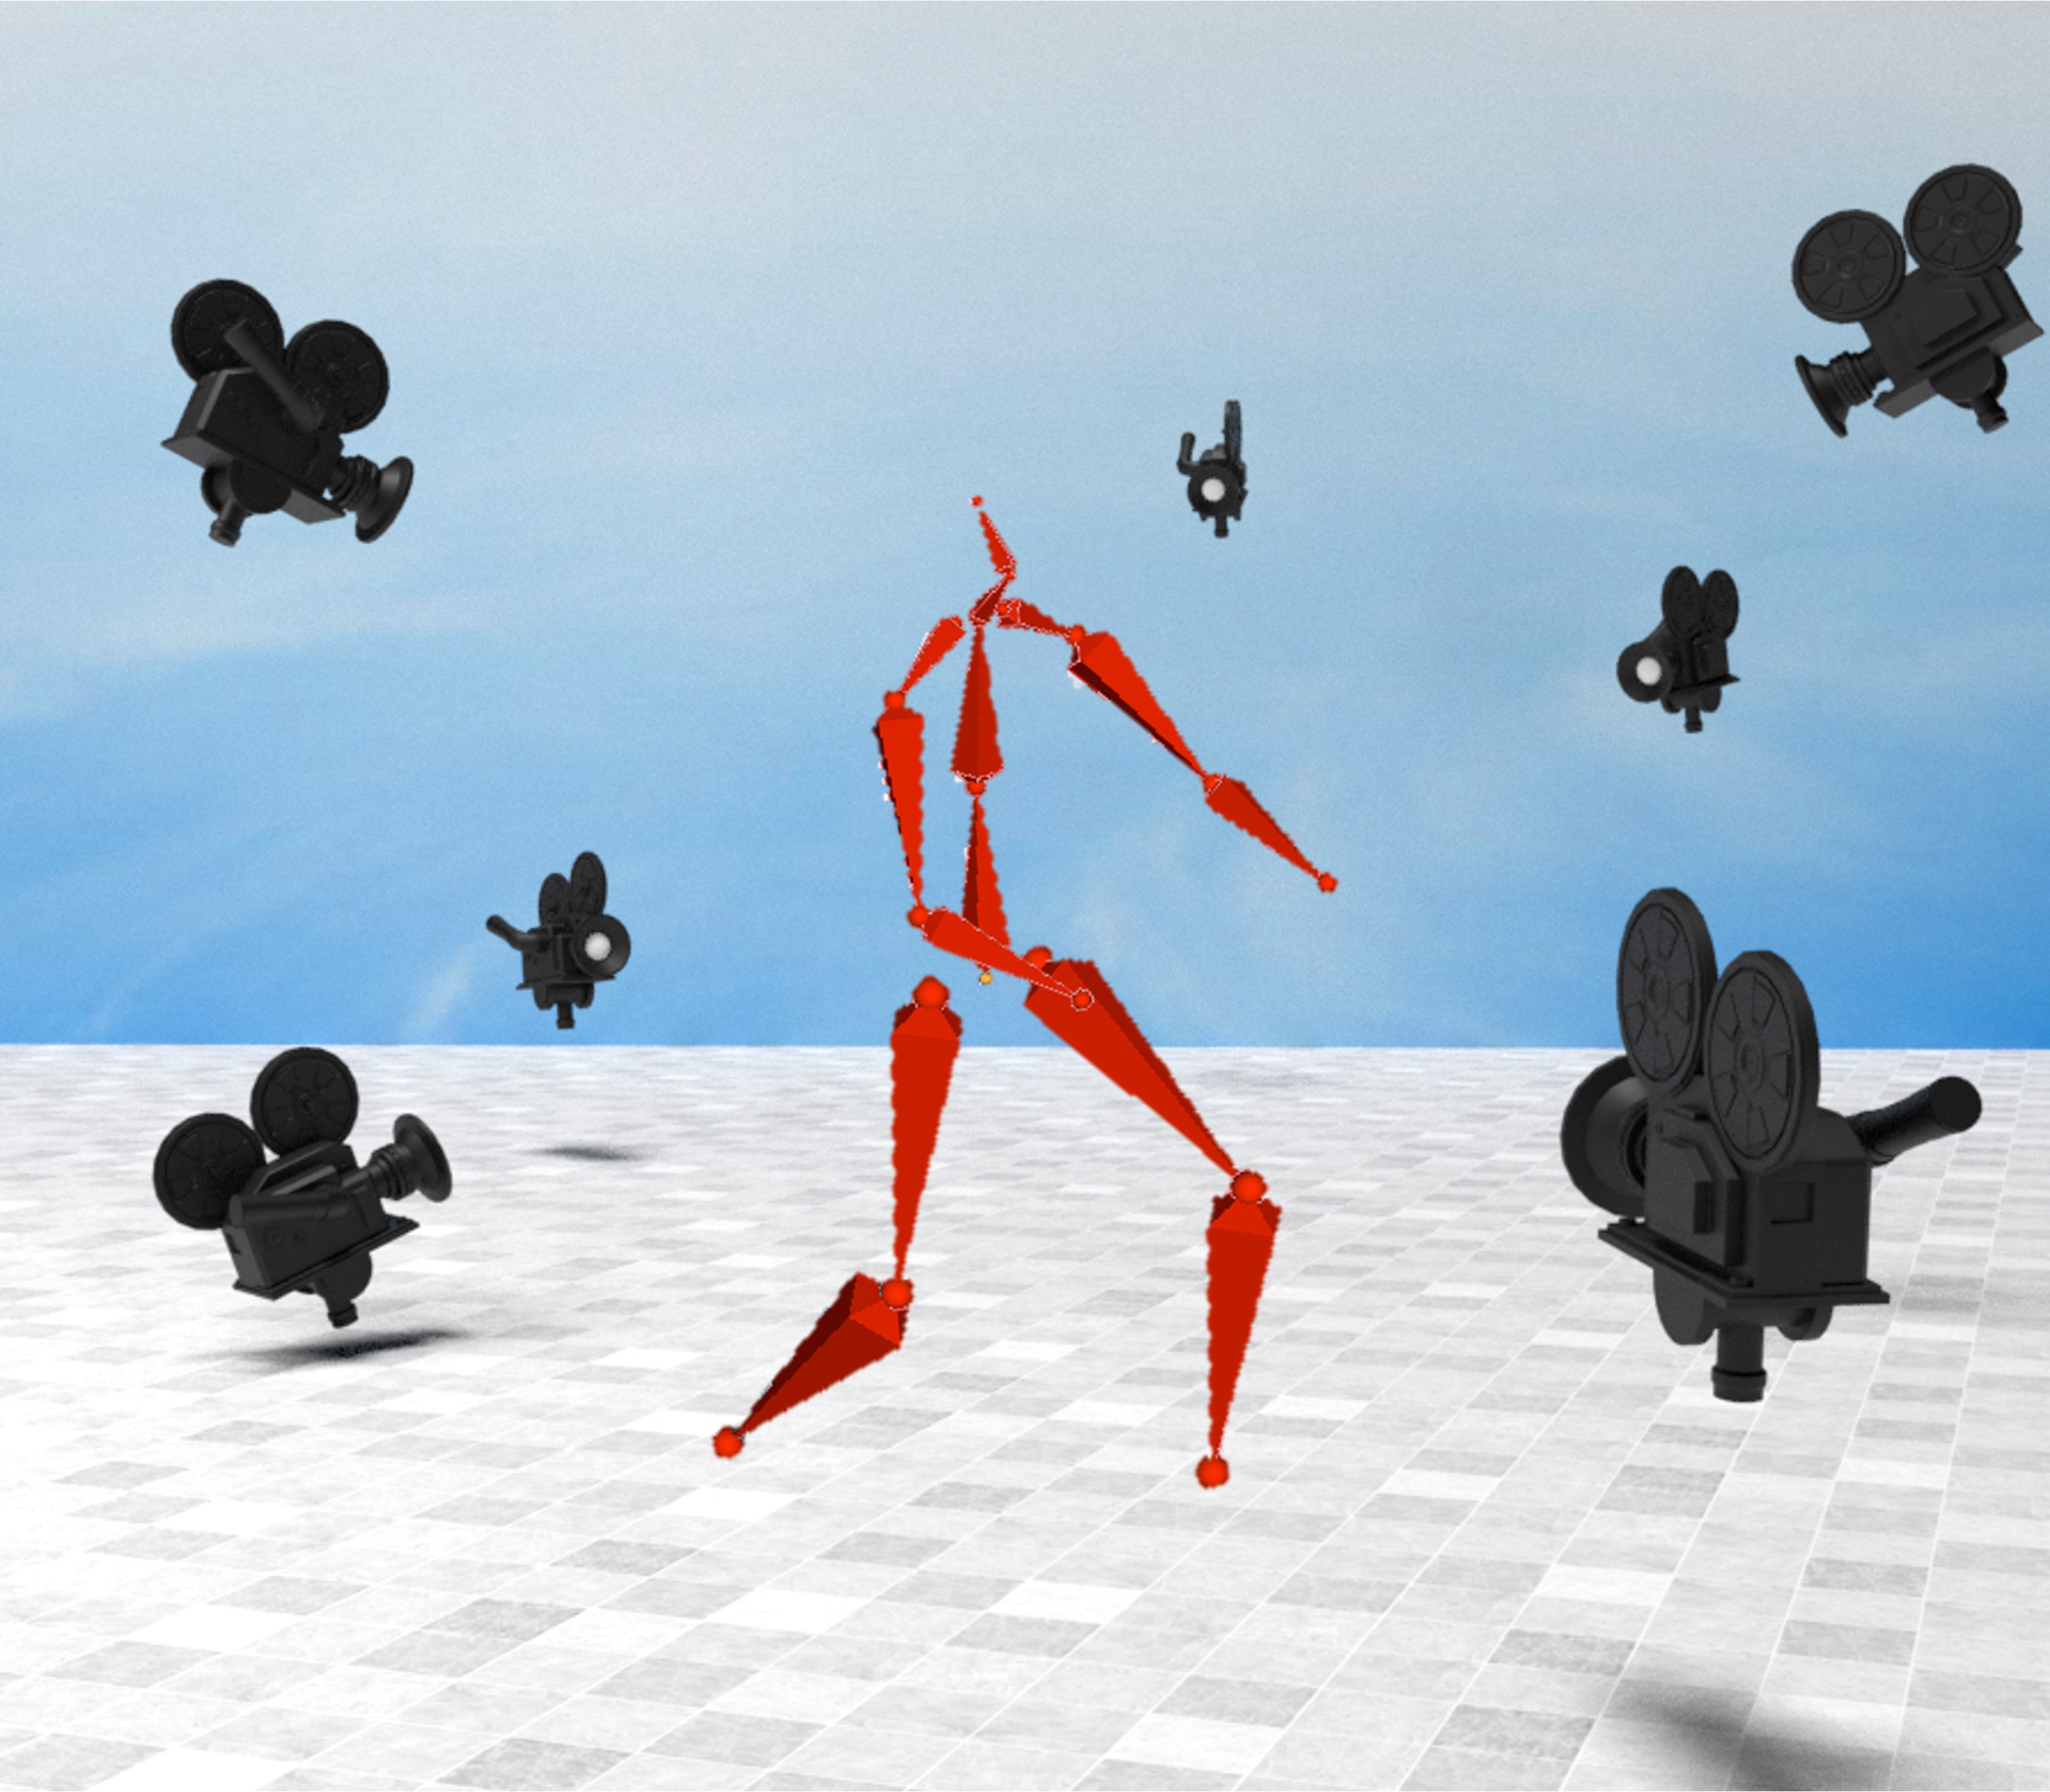
\includegraphics[width=0.3\textwidth]{./images/skeleton_teaser.jpg}
%     % \caption{}
% %   \caption{FLEX reconstructs human motion in environments of multiple cameras, where the camera parameters are unknown.}
% %   \caption{Human motion, captured by multiple cameras.}
%   \label{fig:skeleton_cameras}
% \end{wrapfigure}

\begin{wraptable}{r}{0.48\textwidth}
\setlength{\abovecaptionskip}{-5pt plus 3pt minus 2pt}
\setlength{\belowcaptionskip}{-24pt plus 3pt minus 2pt}

% \begin{table}[h]
\ifeccv
\caption{
%Protocol \#1 
MPJPE 
%error 
on the Ski-PTZ dataset,
measured for methods trained when extrinsic parameters are \emph{not} given. 
%Legend: 
$(\dagger)$ is self/weakly-supervised. 
%$(*)$ is weakly supervised.
}
\fi
\begin{center}
\begin{tabular}{|c|c|}
\hline
\textbf{Method} & \textbf{MPJPE
%(mm) $\downarrow$ 
} \\
\hline
% \hline
% \multicolumn{2}{|l|}{Multi-view methods cam. param. \textbf{ given} } \\
% \hline
% Epipolar Trans.~\cite{he2020epipolar} & 34.2 \\
% TransFusion~\cite{ma2021transfusion} & \textbf{31.6} \\
% \hline
% \hline
% \multicolumn{2}{|l|}{Multi-view methods cam. param. \textbf{ not given} }\\
% \hline
CanonPose~\cite{wandt2020canonpose} ($\dagger$) & 128.1 \\
% \hline
Chen \etal~\cite{chen2021deductive} ($\dagger$) & 99.4 \\
% \hline
Ours & \textbf{65.5} \\
\hline
\end{tabular}
\end{center}

\ifeccv
\else
\caption{Protocol \#1 MPJPE error on the Ski-PTZ dataset,
measured for methods that are trained when extrinsic parameters are \textbf{not} given. 
Legend: $(\dagger)$ is self-supervised. 
$(*)$ is weakly supervised.}
\fi


\label{tab:ski_quantitative}
% \end{table}

\setlength{\abovecaptionskip}{-50pt plus 3pt minus 2pt}
\setlength{\belowcaptionskip}{-0pt plus 3pt minus 2pt}
\caption*{}

\end{wraptable}

In addition to the comprehensive comparison on the Human3.6 dataset, 
in \Cref{tab:ski_quantitative} we show a quantitative comparison on the Ski-Pose PTZ-Camera~\cite{ski_ptz} dataset, for methods that are trained when camera parameters are \emph{not} given.
These methods are comparable in settings that lack extrinsic parameters because they estimate them. 
However, since they still use (estimated) parameters, they are not ep-free.
FLEX leads the table with a large gap.
This gap is mostly because parameter estimation induces an inevitable inaccuracy, and partially because the compared models are self/semi-supervised. 

\begin{table}[t!]
\setlength{\abovecaptionskip}{-5pt plus 3pt minus 2pt}
\setlength{\belowcaptionskip}{-5pt plus 3pt minus 2pt}

    \hfill
    \begin{minipage}{.35\linewidth}
        \centering
        % \captionsetup{justification=centering}    
        \caption{Smoothness, measured by acceleration error ($mm/s^2$), on Human3.6M.\\
        ($\star$):~2D pose from \cite{iskakov2019learnable}.\hfill\\ ($\bullet$):~ground-truth 2D poses.}
        \begin{center}
\begin{tabular}{|c|c|}
\hline
\ifeccv \else \kern-3pt \fi
\textbf{Method} & \textbf{Acc. Err.}$\ \downarrow$ \\ \hline
VIBE\cite{kocabas2020vibe} & 18.3 \\ \hline
MEVA\cite{luo20203d} & 15.3 \\ \hline
HMMR\cite{kanazawa2019learning} & 9.1 \\ \hline
TCMR\cite{choi2021static} & 5.3 \\ \hline
Iskakov\cite{iskakov2019learnable} & 3.9\\ \hline
Shi\cite{shi2020motionet}  & 3.6($\star$) / 2.0($\bullet$) \\ \hline
FLEX  & \textbf{1.6}($\star$) / \textbf{0.9}($\bullet$) \\ \hline

\end{tabular}
\end{center}



%%%%%%%%%%% ECCV POSTER TABLE %%%%%%%%%%% 
% \begin{center}
% \begin{tabular}{|c|c|}
% \hline
% \ifeccv \else \kern-3pt \fi
% \textbf{Method} & \textbf{Acc. Err.}$\ \downarrow$ \\ \hline
% VIBE[4] & 18.3 \\ \hline
% MEVA[5] & 15.3 \\ \hline
% HMMR[5] & 9.1 \\ \hline
% TCMR[6] & 5.3 \\ \hline
% Iskakov[3] & 3.9\\ \hline
% Shi[7] & 3.6 \\ \hline
% Ours  & \textbf{1.6} \\ \hline

% \end{tabular}
% \end{center}










        \ifeccv
        \else
        \caption{Smoothness, measured by acceleration error ($mm/s^2$), on Human3.6M.\\
        ($\star$):~2D pose from \cite{iskakov2019learnable}.\hfill\\ ($\bullet$):~ground-truth 2D poses.}
        \fi
        \label{tab:acc_error}
    \end{minipage}%
    \hfill
    \begin{minipage}{.36\linewidth}
      \centering
        % \captionsetup{justification=centering}    
        \caption{Attention impact.\\ TE: Transformer Encoder.\hfill \\MHA: Multi-head Attention.\hfill\\ $l$: no. of stacked layers.\\ $h$: no. of attention heads.}
        % \begin{wraptable}{r}{4.5cm}
\begin{center}
\begin{tabular}{|c|c|}
\hline

\textbf{Method} & \textbf{MPJPE} \\

\hline
Conv. layer & 31.9 \\
\hline
TE - 1$l$, 64$h$ & 30.9 \\
\hline
TE - 2$l$, 64$h$ & 37.8 \\
\hline
MHA - 128$h$ & 30.5 \\
\hline
MHA - 64$h$ & \textbf{30.2} \\
\hline
MHA - 32$h$ & 30.6 \\
\hline
MHA - 16$h$ & 30.9 \\
\hline

\end{tabular}
\end{center}
% \caption{The impact of multi-view fusion architecture. Legend: TE - Transformer Encoder. MHA - Multi-head Attention. $l$ refer to no. of stacked layers. $h$ refer to no. of heads in attention layer.}
% \label{tab:fusion_arch}
% \end{wraptable}

        \label{tab:fusion_arch}
    \end{minipage}
    \hfill
    \hphantom{.} % this non printed text makes the \hfill in the previous line work
    
\setlength{\abovecaptionskip}{-35pt plus 3pt minus 2pt}
\setlength{\belowcaptionskip}{-0pt plus 3pt minus 2pt}
\caption*{}

\end{table}

A known strength of predicting rotation angles rather than locations, is the \emph{smoothness} of predicted motion. 
% In \Cref{tab:acc_error} we compare the smoothness of our work against others, using a metric proposed by Kanazawa \etal~\cite{kanazawa2019learning}. Smoothness is quantified by the acceleration error of each joint. Notice our work leads the table by a large margin.
In \Cref{tab:acc_error} we show that FLEX's smoothness result outperforms others by a large margin. Following Kanazawa \etal~\cite{kanazawa2019learning}, we measure smoothness using the acceleration error of each joint. 

%%%%%%%%%%%%%%%%%%%%%%%%%%%%%%%%%%%%%%%%%%%%%%%%%%%%%%%%%%%%%%%%%%%%%%%%%%

\paragraphtinyvert{Qualitative results}


In the following figures we show rigs, that is, bone structure 
%in frames 
from reconstructed animation videos, selecting challenging %postures and 
scenes. Videos of the reconstructed motions are  
\ifanonymous{provided \iftog{as well,}\else{in the sup. mat.,}\fi}
\else{available on our project page,}
\fi
presenting the smoothness of motion and the naturalness of rotations. 
\Cref{fig:football_teaser,fig:quality_h36,fig:ski_ptz_qualitative}
 show scenes from the KTH Multi-view Football II~\cite{footballDS}, the Human3.6M~\cite{h36m_pami,IonescuSminchisescu11} and the Ski-Pose PTZ-Camera~\cite{ski_ptz} datasets, respectively. 
Each row depicts three views of one time frame. To the right of each image, we place a reconstructed rig, which is sometimes zoomed in for better visualization. 
%KTH results are computed by using the model that was trained on Human3.6M, without re-training it on this one, demonstrating that FLEX generalizes well. 
Notice the occluded and blurry scenes in the football figure (\ref{fig:football_teaser}). The KTH Football dataset is filmed using dynamic (moving) cameras, 
a setting where extrinsic parameters are rarely given, thus disqualifying methods that require camera parameters.
%hence it is challenging for other multi-view algorithms to reconstruct pose/motion over it without using the given camera parameters.
Our algorithm is agnostic to the lack of camera parameters and attains good qualitative results. 

%\brchange{}{\textbf{REMOVED FROM HERE KTH FIGURE WITH BLURRED WAVING HAND TO SUP.MAT. \ref{fig:quality_football_hand_wave}}}
% In Figure \ref{fig:quality_football_hand_wave} we show that our algorithm is able to grasp fine details. The player's left hand cannot be seen in the center view and is blurred in the left views. Yet, our model accurately reconstructs it.
In \Cref{fig:competitors} we show qualitative results of FLEX, compared to current non ep-free  multi-view state-of-the-art \cite{iskakov2019learnable}, and to our monocular baseline~\cite{shi2020motionet}. 
Note that the method in \cite{iskakov2019learnable} produces unnatural poses such as a huge leg in the first row and a backward-bent elbow in the last row. 

\begin{figure}[t]
\setlength{\abovecaptionskip}{5pt plus 3pt minus 2pt}
\setlength{\belowcaptionskip}{-5pt plus 3pt minus 2pt}
\centering
\begin{minipage}[b]{0.48\linewidth}
    \centering
    % 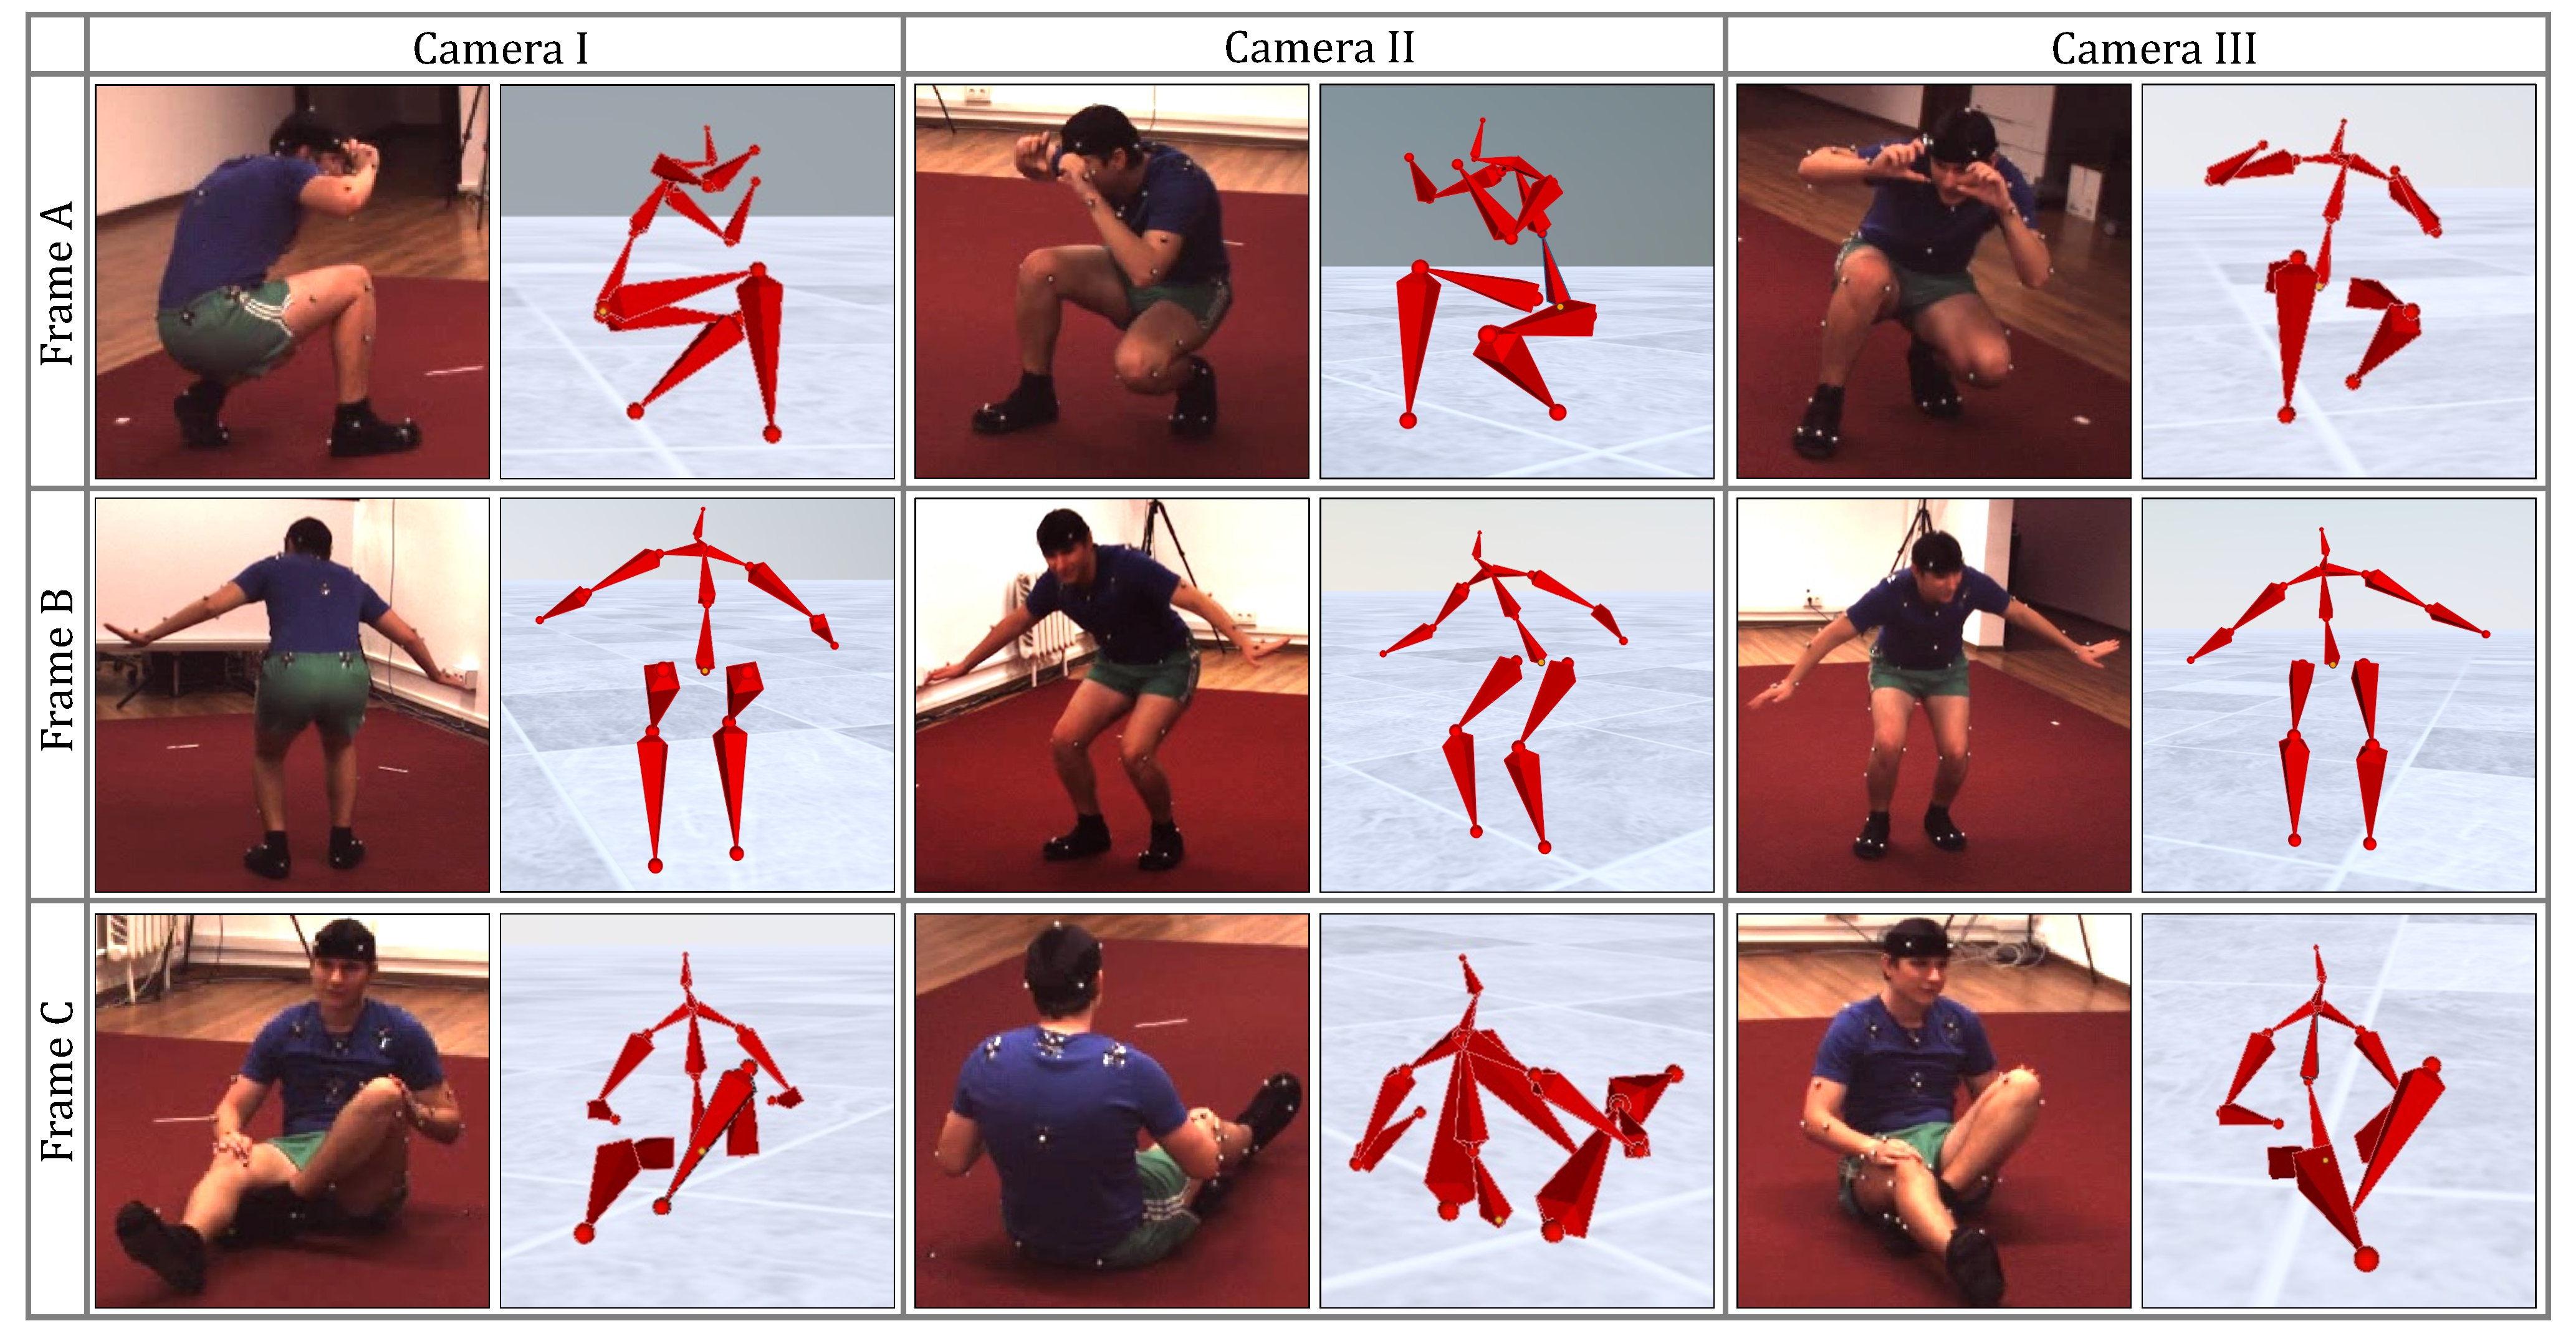
\includegraphics[width=\textwidth]{./images/H36M_results.pdf}
    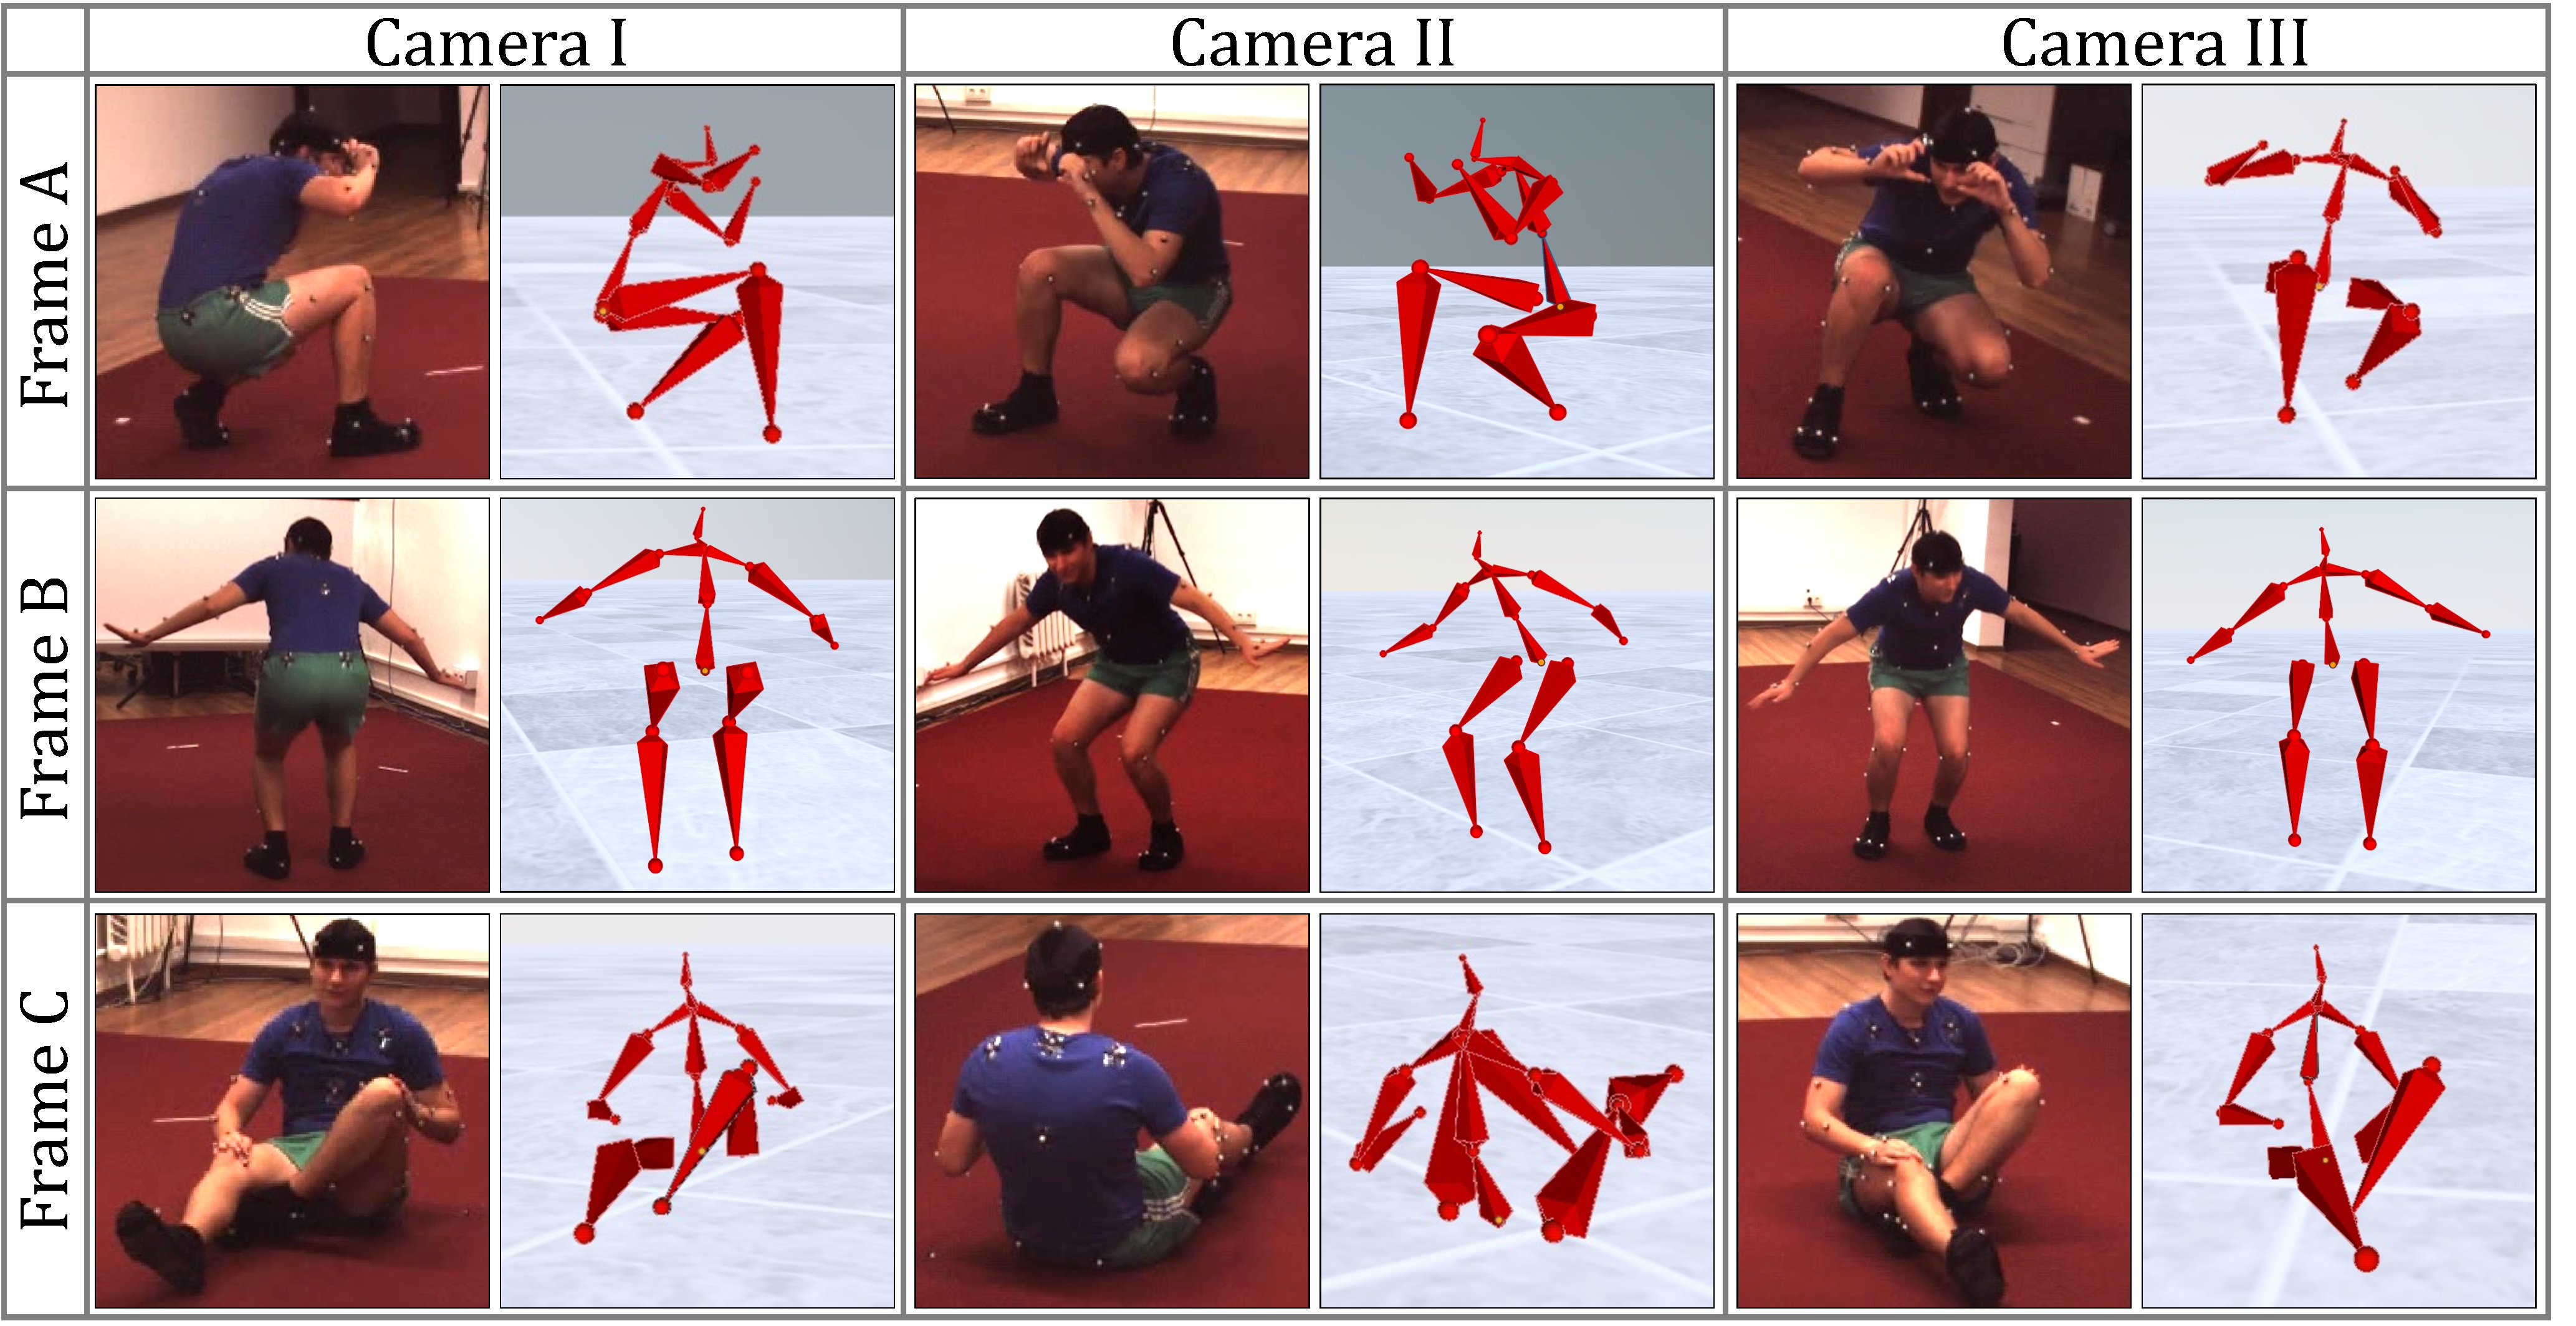
\includegraphics[width=\textwidth]{./images/H36M_results_big_font.pdf}
    \caption{Our results on videos from the Human3.6M dataset.}
    \label{fig:quality_h36}
\end{minipage}
\hfill
\begin{minipage}[b]{0.48\linewidth}
    \centering
    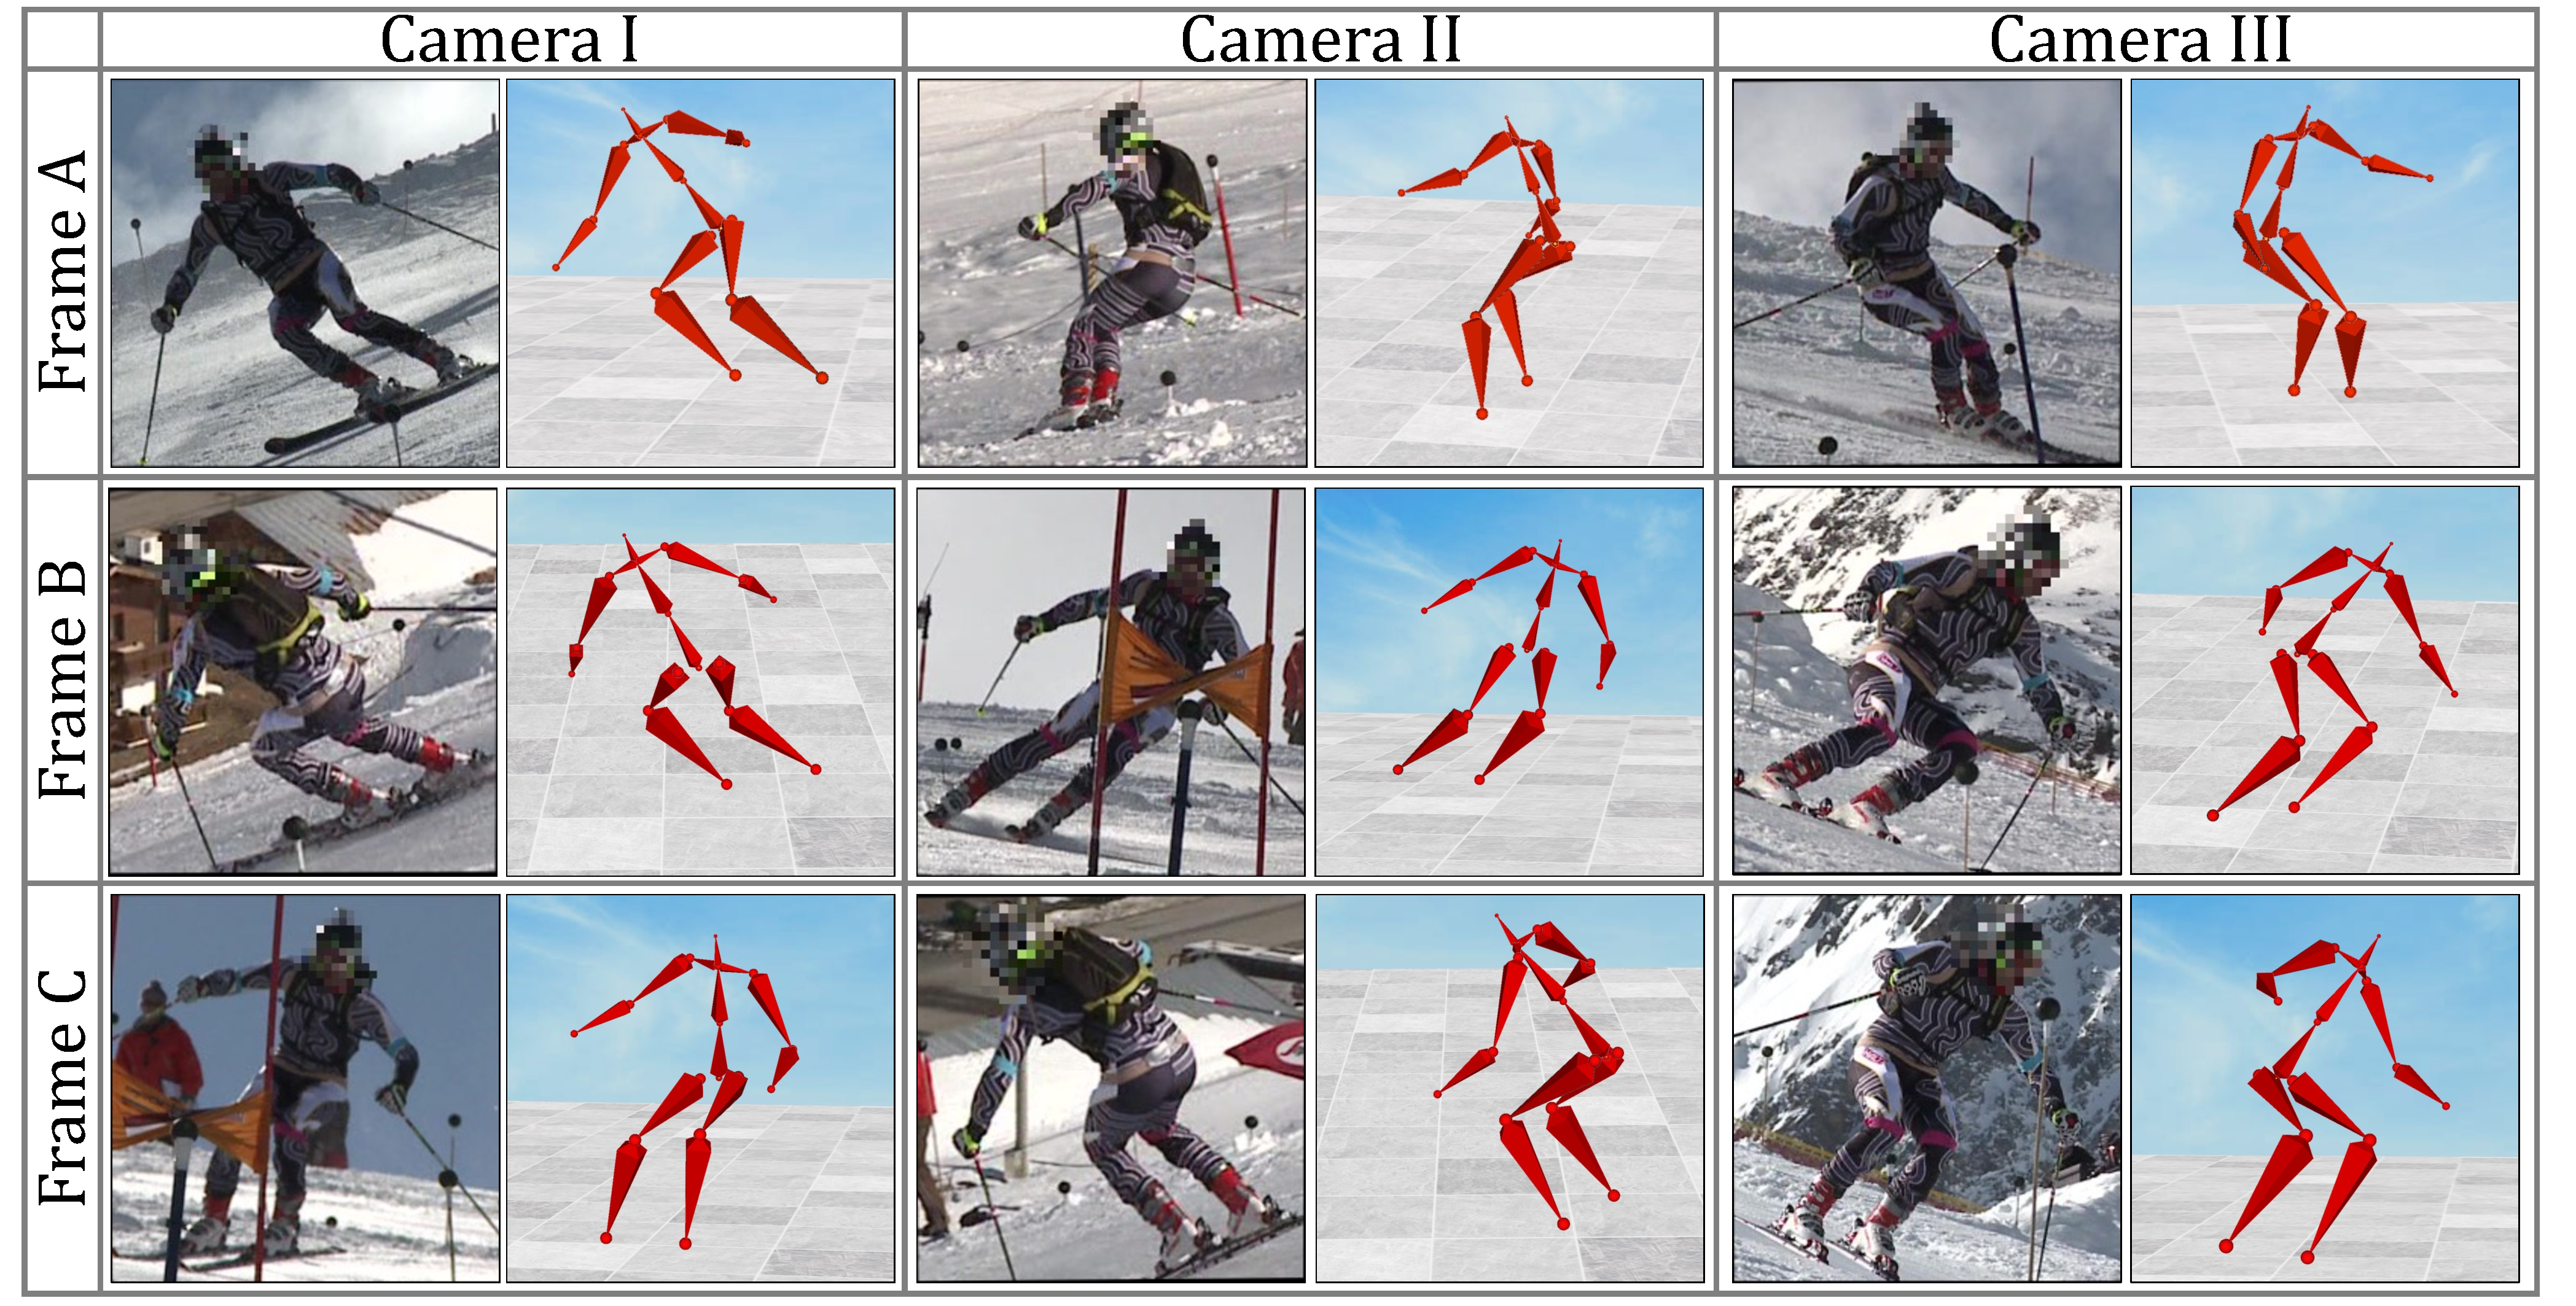
\includegraphics[width=\textwidth]{./images/Ski_results.pdf}
    \caption{Our results on videos from the Ski-Pose PTZ-Camera dataset.}
    \label{fig:ski_ptz_qualitative}
\end{minipage}
\end{figure}


\begin{figure}[t]
\setlength{\abovecaptionskip}{5pt plus 3pt minus 2pt}
\setlength{\belowcaptionskip}{-15pt plus 3pt minus 2pt}
\centering
\begin{minipage}[b]{0.68\linewidth}
    \centering
    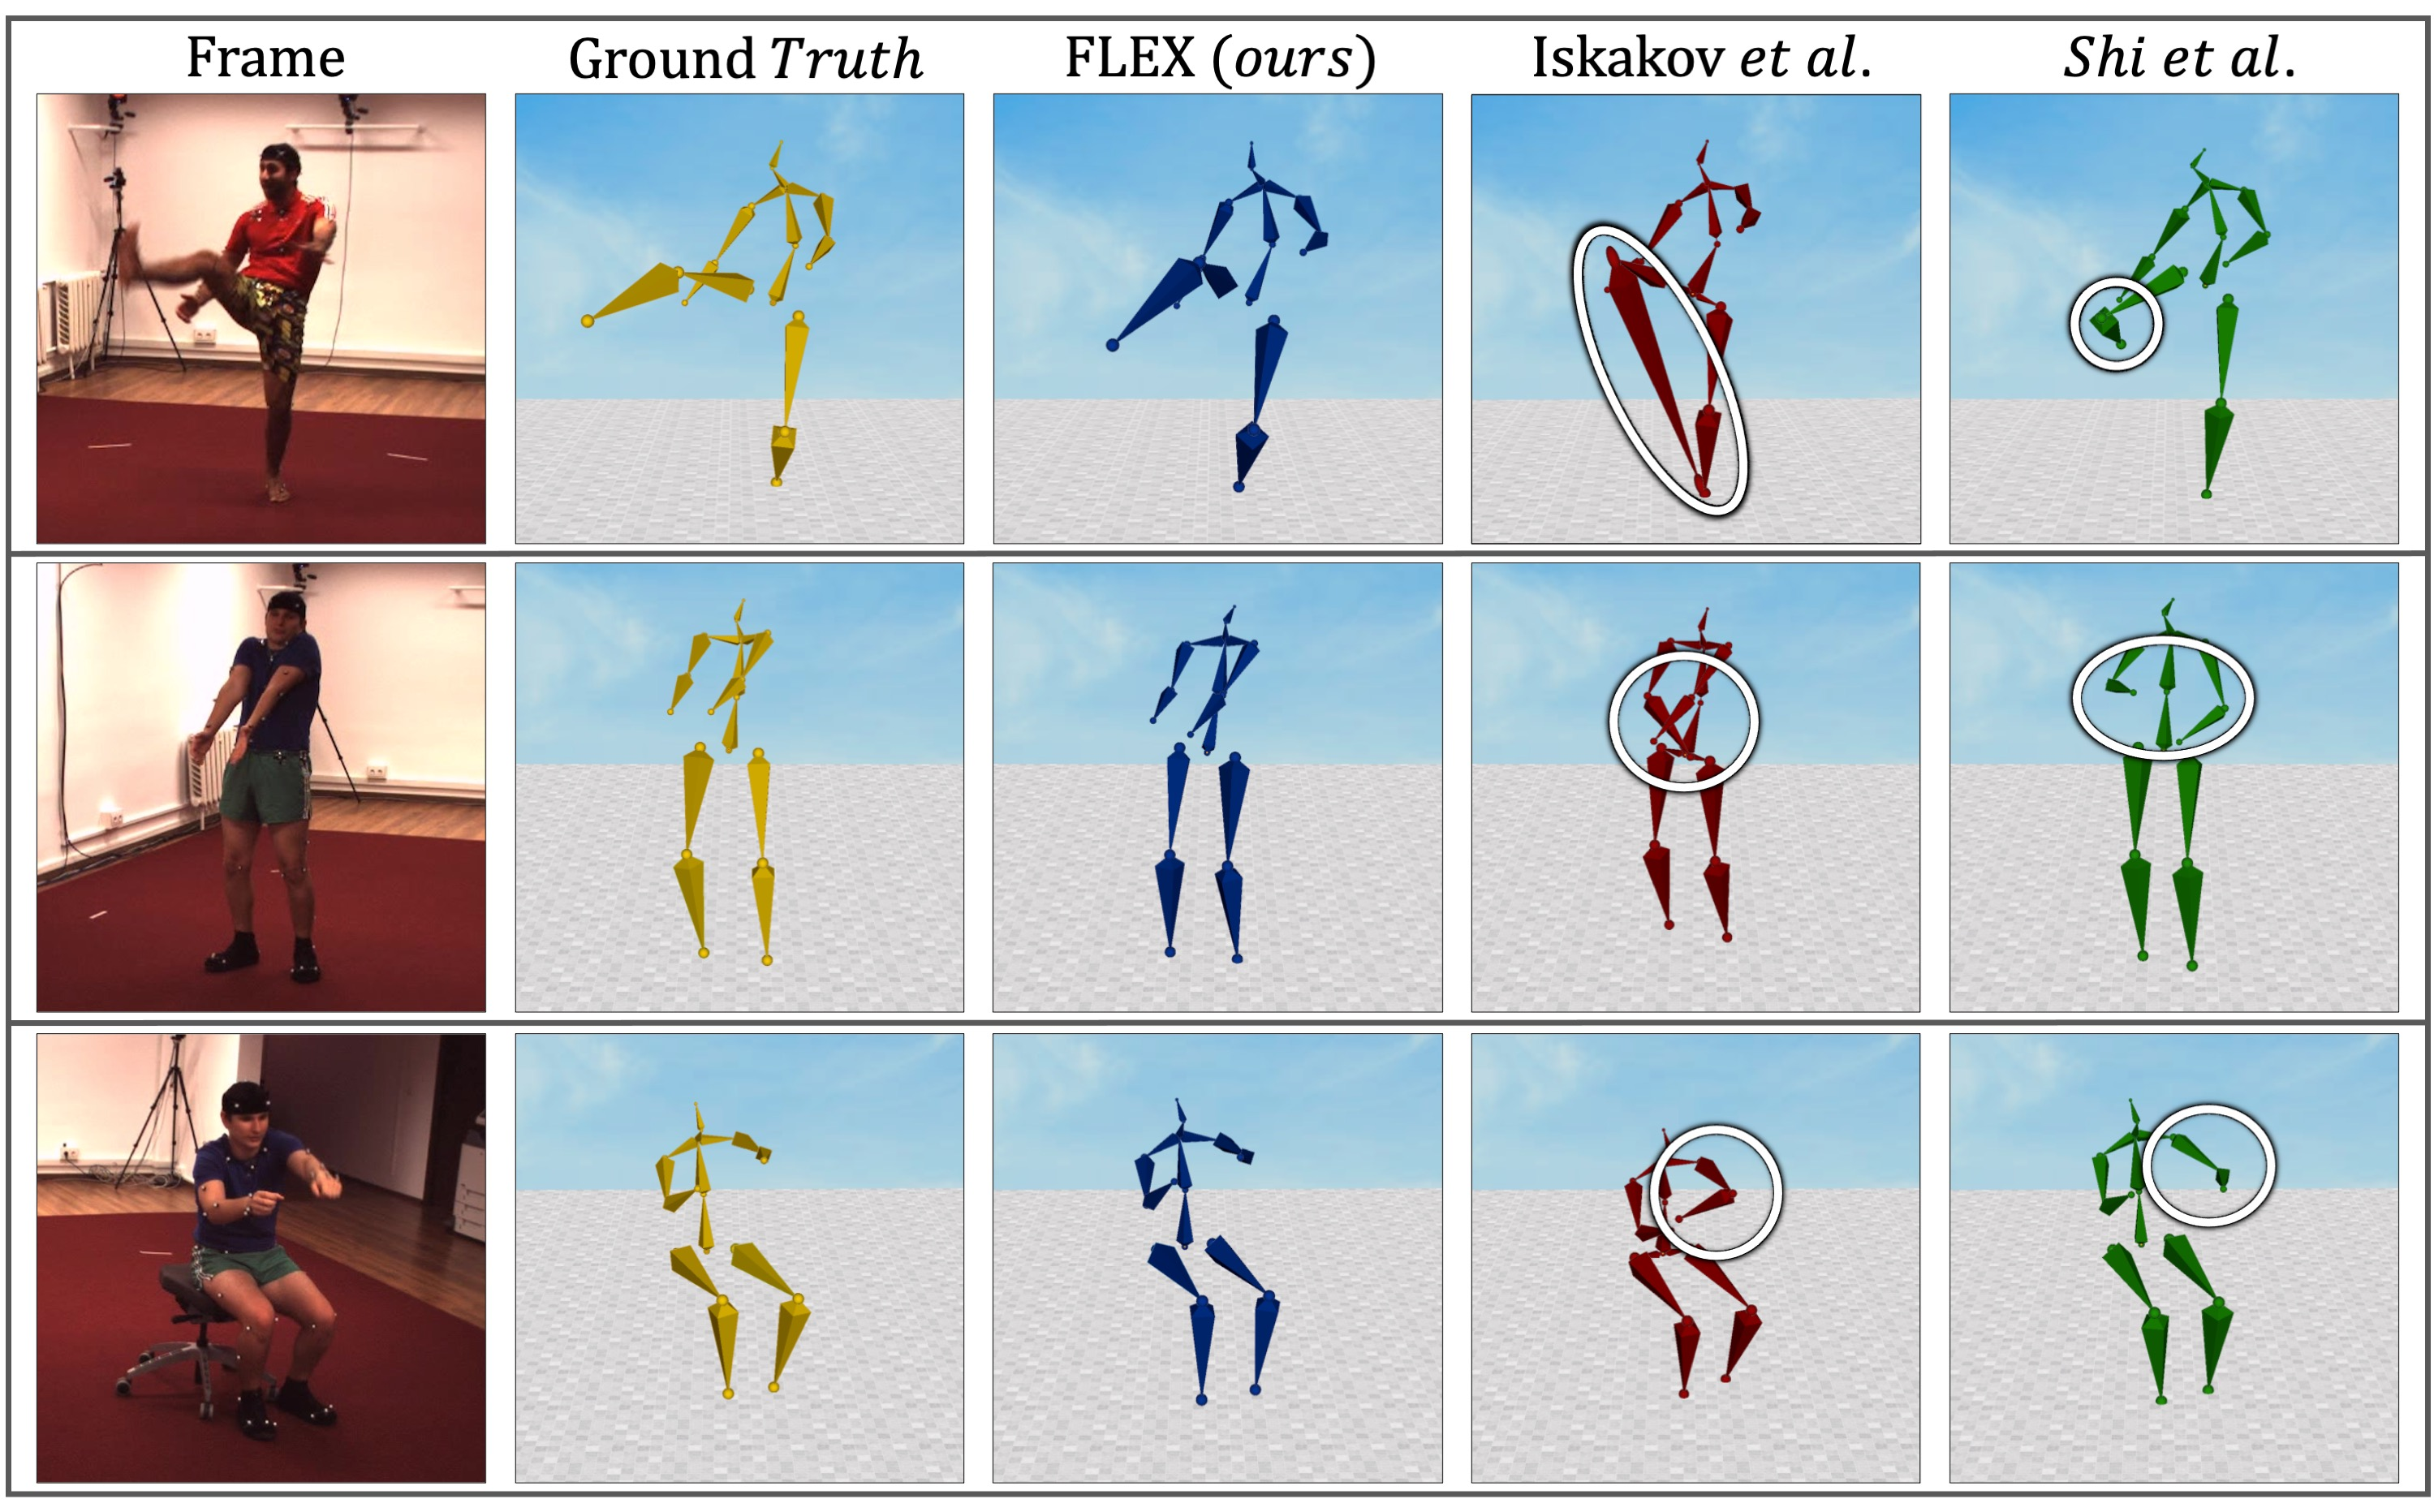
\includegraphics[width=\textwidth, height=5.0cm]{./images/competitors_grid.jpg}
    \caption{Qualitative comparison of our work vs. non ep-free state-of-the-art (Iskakov \etal~\cite{iskakov2019learnable}) and vs. our single-view baseline (Shi \etal~\cite{shi2020motionet}).}
    \label{fig:competitors}
\end{minipage}
\hfill
\begin{minipage}[b]{0.27\linewidth}
    \centering
    % \includegraphics[width=\textwidth]{./images/root_positions_color_vertical.jpg}
    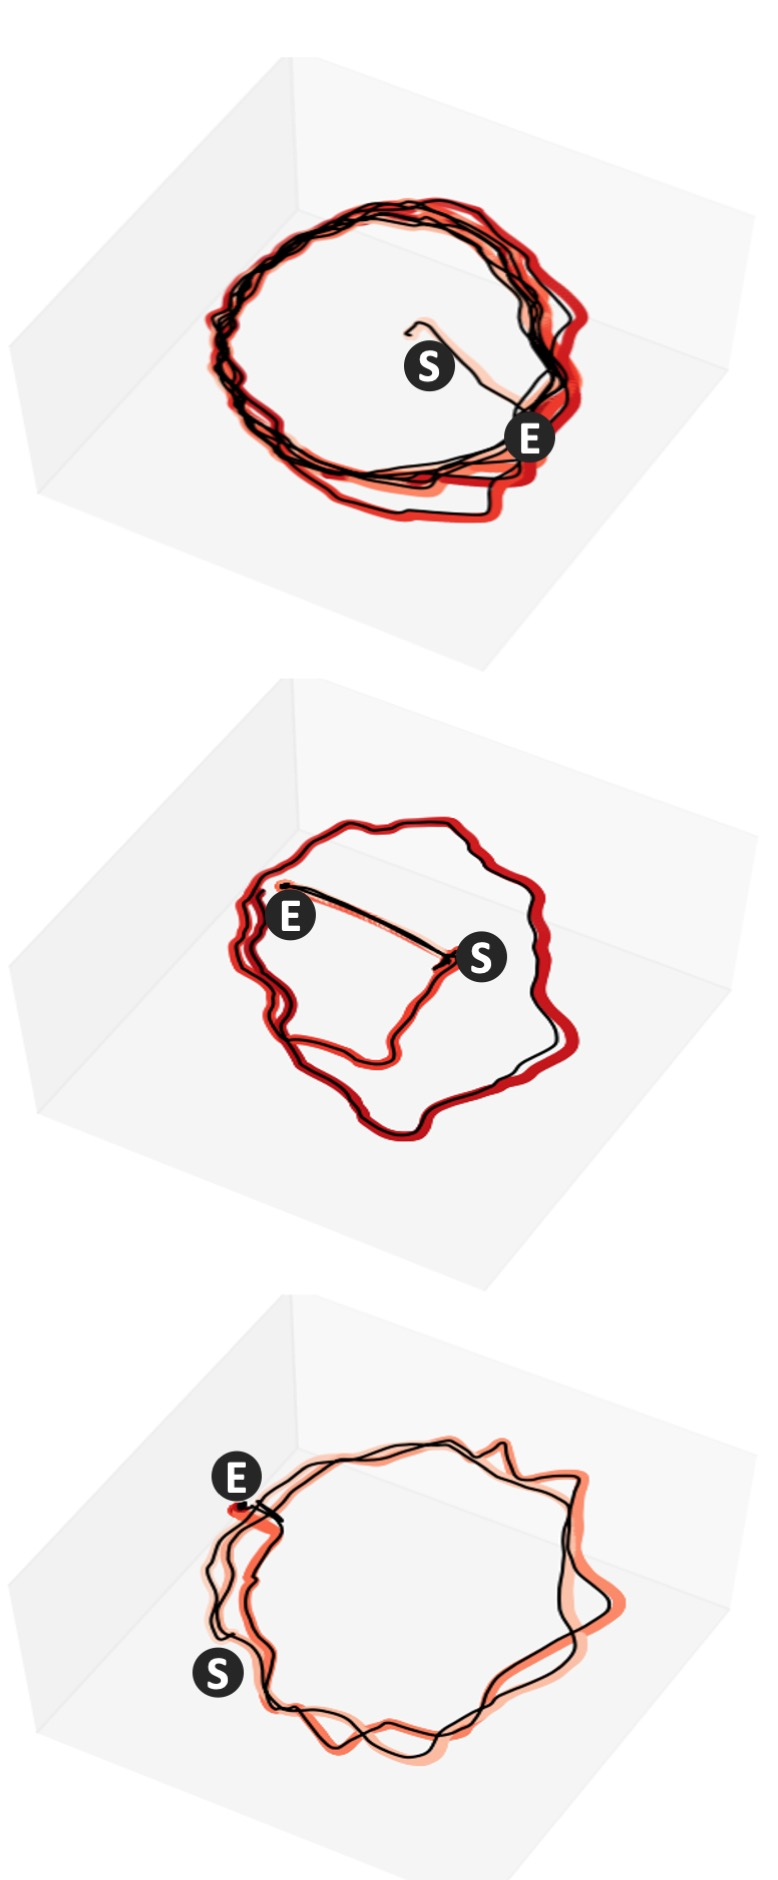
\includegraphics[width=0.8\textwidth,height=5.0cm]{./images/root_color_vert2.jpg}
    \caption{Global root position. Ground-truth is in thin black.}
    \label{fig:root_pos}
\end{minipage}
\end{figure}


\begin{figure*}[htb]
\setlength{\abovecaptionskip}{5pt plus 3pt minus 2pt}
\setlength{\belowcaptionskip}{-15pt plus 3pt minus 2pt}
\centering
% \includegraphics[width=\linewidth]{./images/Fight_results_with_circles.pdf}
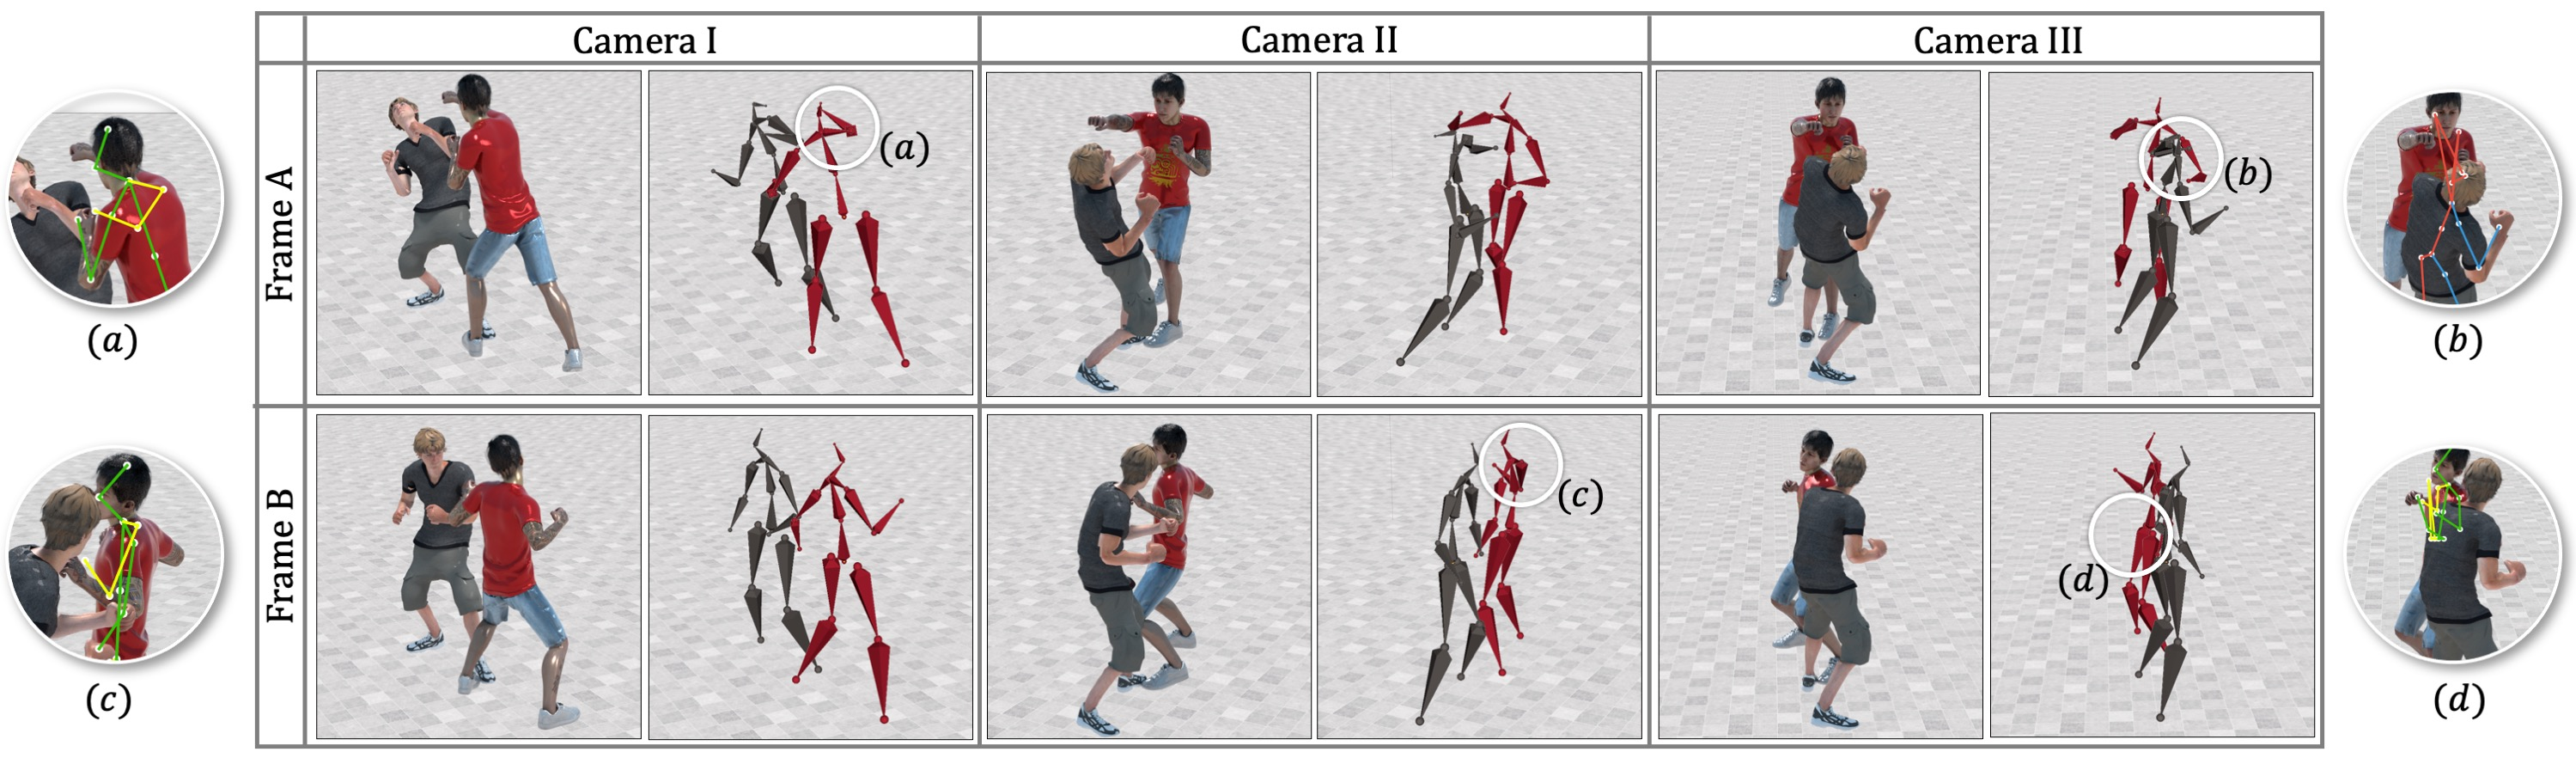
\includegraphics[width=\linewidth]{./images/Fight_results_with_circles_2_ROWS_new_design.jpg}
\caption{Results on multi-person synthetic videos.
% Our method reconstructs correct 3D motion although it takes inaccurate 2D joints for input. 
%Let \emph{gray fighter} and \emph{red fighter} denote the fighter wearing a gray and a red shirt, respectively. 
\sr{In the zoomed-in circular images we depict 2D pose estimations, which are erroneous due to occlusion. A matching circle in the center rectangular image shows that 
our method reconstructs correct 3D motion although it takes inaccurate 2D joints for input. 
% the motion reconstruction has not been affected by the erroneous 2D estimation.
}
%Several error examples are depicted in the zoomed-in circular insets: % (a) The right hand of the red fighter is self-occluded, so its 2D pose conveys a large error;
% (b) The nose tip of the gray fighter is erroneously detected next to the right eye of the red fighter, and his left arm is mismatched;
% (c) Erroneous 2D pose estimation of the red fighter's right hand;
% (d) The red fighter is mostly occluded; hence the 2D joint estimation of his body is a 
% blunder. 
} 
\label{fig:fight_results_with_circles}
\end{figure*}


\paragraphtinyvert{Multi-person captured by dynamic cameras} 
We evaluate our algorithm on
a setting with dynamic cameras, with multi-person scenes introducing
severe inter-person occlusions.
% multi-person scenes, where severe inter-person occlusions are present, and the cameras are dynamic.
Recall that the term \emph{dynamic} refers to moving cameras that occasionally change their location and rotation.
%
There are several multi-view datasets. Most of them are not fully dynamic: Human3.6M~\cite{h36m_pami,IonescuSminchisescu11}, CMU Panoptic~\cite{CMU:mocap} and TUM Shelf $\&$ Campus~\cite{campus_shelf} contain static scenes only, while Tagging~\cite{tagging_dataset} and Ski-Pose PTZ-Camera~\cite{ski_ptz} contain  rotating cameras whose locations are fixed. KTH~\cite{footballDS} is fully dynamic, but it is too blurry and does not provide ground-truth for all subjects.
Despite its limitations, we use the KTH dataset for qualitative analysis, but we cannot use it for thorough research.
To mitigate the lack of a dynamic dataset, we generate synthetic videos using animated characters downloaded from Mixamo~\cite{mixamo}, an online dataset of character animation. Then, we generate video sequences of two interacting characters using Blender~\cite{blender}, which is a 3D creation suite. The newly created data is available on our project page.
Our "synthetic studio" is illustrated at the \ifarxiv{appendix}\else{sup. mat.}\fi, where two interacting figures are video-filmed by multiple dynamic cameras.
Using Blender, we obtain a rendered video stream from the view angle of each synthetic camera. 
Recall that the input to our algorithm is 2D joint locations, hence it is agnostic to the video appearance, and to whether the input image is real or synthetic.

The 2D backbone we use over the rendered video sequences is Alphapose~\cite{alphapose}, a state-of-the-art multi-person 2D pose estimator.
Once obtaining the 2D joint locations, we use a na\"ive heuristic, which is not part of the suggested algorithm, to associate each detected person with its ID: for each frame, we associate the detected 2D pose with the one that is geometrically closest to it in the previous frame. 
% This heuristic is not part of the suggested algorithm. 
%It simply uses the assumption that the motion between two consecutive frames is minimal. Thus, for each frame, we associate the detected 2D pose with the one that is geometrically closest to it in the previous frame.
In \Cref{fig:fight_results_with_circles} we depict qualitative results of two boxers. We emphasize several viewpoints where the 2D estimator attains large errors. Yet, FLEX compensates for these errors by fusing multi-view information. In the \ifarxiv{appendix }\else{sup. mat. }\fi we show additional characters and the predicted 2D pose for all the viewpoints.

%%%%%%%%%%%%%%%%%%%%
\paragraphtinyvert{Global position}

In \Cref{fig:root_pos} we draw the global position of the scaled predicted root joint along time.
Ground-truth is depicted using a thin black curve, and our prediction is an overlay on top of it, changing from light to dark as time progresses. The start and the end of each trajectory are signaled by the letters S and E, respectively.
Depicted motions are evaluated on the test set of Human3.6M, on the motions of walking, talking on the phone, and eating.
Note that our predictions almost completely overlap the ground-truth curve. 
Recall we use weak perspective to bypass dependency on intrinsic parameters, resulting in up-to-scale global position accuracy. 
\sr{Quantitatively, our MPJPE on the H36M validation
set is $118mm$, outperforming Iskakov \etal~\cite{iskakov2019learnable} (perturbed by 3\%) that attain $123mm$. The other ep-free work \cite{chu_and_pan_semisupervised} does not solve global locations.}
%\bg{FLEX absolute positions MPJPE results to 118mm error, while Iskakov \etal~\cite{iskakov2019learnable} perturbed with noise (as explained in Quantitative Results section) produces an MPJPE of 123mm. The other ep-free work \cite{chu_and_pan_semisupervised} does not solve global locations whatsoever.}

% {
% \color{red}
% 
\begin{table}[tb]
\color{red}
\begin{center}
\caption{Global MPJPE error on Human3.6M.
Legend:$(*)$ is a non ep-free algorithm.}
\begin{tabular}{|c|c|}
\hline
\textbf{Method} & \textbf{MPJPE} \\ \hline
\makecell{Iskakov\cite{iskakov2019learnable}$(*)$ \\ param. perturb by 3\%} & 123 \\ \hline
FLEX & \textbf{118} \\ \hline

\end{tabular}
\label{tab:global_mpjpe}
\end{center}


\end{table}

% }

%%%%%%%%%%%%%%%%%%%%
\paragraphtinyvert{Ablation study}

\ifeccv{
    \begin{table}[t]
\setlength{\abovecaptionskip}{0pt plus 3pt minus 2pt}
\setlength{\belowcaptionskip}{10pt plus 3pt minus 2pt}
    \caption{Ablation studies: The impact of (a) Number of views; (b) 2D backbone, and (c) Fusion method \sr{(refer to the sup. mat. for details regarding fusion)}.}
    %The impact of various fusion methods with 2D GT input. Note that processing all views together with an early fusion as done in FLEX outperforms the other variations by a large margin.}
    \begin{minipage}{.32\linewidth}
\setlength{\abovecaptionskip}{0pt plus 3pt minus 2pt}
\setlength{\belowcaptionskip}{-10pt plus 3pt minus 2pt}
        \centering
        % \caption{No. of views impact.}
        \caption*{\small(a)}
        % \begin{table}[tb]
% % \begin{wraptable}{r}{4.5cm}
% \begin{center}
% \begin{tabular}{|c|c|c|}
% \hline
% %\makecell{\textbf{2D from} $\rightarrow$ \\ \textbf{\#Views}\downarrow$}& \textbf{GT } & \textbf{\cite{iskakov2019learnable}}\\
% \makecell{\textbf{2D from$\rightarrow$} \\ \textbf{\#Views$\downarrow$}} & \textbf{GT } & \textbf{\cite{iskakov2019learnable}}\\

% \hline
% 1 & 47.7 & 56.3 \\
% \hline
% 2 & 33.9 & 41.4\\
% \hline
% 3 & 27.8 & 34.7 \\
% \hline
% 4 & 24.8 & 30.18 \\
% \hline
% \end{tabular}
% \end{center}
% \caption{Varying number of views.}
% \label{tab:num_views}
% % \end{wraptable}
% \end{table}

% \begin{wraptable}{r}{4.5cm}
\begin{tabular}{|c|c|c|}
\hline
%\makecell{\textbf{2D from} $\rightarrow$ \\ \textbf{\#Views}\downarrow$}& \textbf{GT } & \textbf{\cite{iskakov2019learnable}}\\
\multirow{2}{*}{\textbf{\#Views}} & \multicolumn{2}{c|}{\textbf{2D backbone}} \\ \cline{2-3} 
 & \rule{0pt}{2ex}\textbf{GT } & \textbf{\cite{iskakov2019learnable}}\\
% removed "\kern-3pt" from before and after "\textbf{\#Views}"
\hline
1 & 47.7 & 56.3 \\
\hline
2 & 33.9 & 41.4\\
\hline
3 & 26.3 & 34.6 \\
\hline
4 & \textbf{22.9} & \textbf{30.2} \\
\hline
\end{tabular}

% \caption{Varying number of views.}
% \label{tab:num_views}
% \end{wraptable}

        \label{tab:num_views}
    \end{minipage}
    \hfill
    \begin{minipage}{.32\linewidth}
\setlength{\abovecaptionskip}{-10pt plus 3pt minus 2pt}
\setlength{\belowcaptionskip}{0pt plus 3pt minus 2pt}
        \centering
        % \caption{2D backbone impact.}
        \caption*{\small(b)}
        % \begin{table}[tb]
% % \begin{wraptable}{r}{4.8cm}
% \begin{center}

% \begin{tabular}{|c|c|}
% \hline
% \textbf{2D backbone} & \textbf{MPJPE }\\
% \hline
% Ground-Truth &24.8\\
% \hline
% OpenPose~\cite{Cao:2018} &38.55\\
% \hline
% CPN~\cite{chen2018cascaded} &31.7\\
% \hline
% \makecell{Iskakov et al.~\cite{iskakov2019learnable} \\ (based on~\cite{xiao2018simple})} &30.18\\
% \hline
% \end{tabular}

% \end{center}
% \caption{Varying 2D pose backbones.}
% \label{tab:2D_backbone}
% % \end{wraptable}
% \end{table}

% \begin{wraptable}{r}{4.8cm}
\begin{center}

\begin{tabular}{|c|c|}
\hline 
\ifeccv \else \kern-3pt \fi
\makecell{\textbf{2D} \\ 
\textbf{backbone}} & 
\ifeccv \else \kern-3pt \fi 
\textbf{MPJPE }
\ifeccv \else \kern-3pt \fi
\\
\hline
% OpenPose~\cite{Cao:2018} &38.55\\
\cite{Cao:2018} &38.6\\
\hline
% CPN~\cite{chen2018cascaded} &31.7\\
\cite{chen2018cascaded} &31.7\\
\hline
% \makecell{Iskakov et al.~\cite{iskakov2019learnable} \\ (based on~\cite{xiao2018simple})} &30.18\\
\cite{iskakov2019learnable} &30.2\\
\hline
GT &\textbf{22.9}\\
\hline

\end{tabular}
%\label{tab:2D_backbone}
\end{center}
% \caption{Varying 2D pose backbones.}
% \end{wraptable}

        \label{tab:2D_backbone}
    \end{minipage}
    \hfill
    \begin{minipage}{.32\linewidth}
\setlength{\abovecaptionskip}{-11pt plus 3pt minus 2pt}
\setlength{\belowcaptionskip}{-21pt plus 3pt minus 2pt}
        \centering
        % \caption{The impact of various fusion methods with 2D GT input.}
        \caption*{\small(c)}
        \begin{center}
\begin{tabular}{|c|c|}
\hline
%\makecell{\textbf{2D from} $\rightarrow$ \\ \textbf{\#Views}\downarrow$}& \textbf{GT } & \textbf{\cite{iskakov2019learnable}}\\
\textbf{Method} & \textbf{MPJPE } \\
\hline
Averaged $K$ views & 36.4 \\
\hline
Late fusion & 31.0 \\
\hline
FLEX & \textbf{22.9} \\
\hline
\end{tabular}
\end{center}
        \label{tab:ablation}
    \end{minipage}
\setlength{\abovecaptionskip}{-35pt plus 3pt minus 2pt}
\setlength{\belowcaptionskip}{-0pt plus 3pt minus 2pt}
\caption*{}
\end{table}

}
\else{
    \begin{table}[t]
    \begin{minipage}{.55\linewidth}
      \centering
      \ifeccv
      \caption{No. of views impact.}
      \fi
        % \begin{table}[tb]
% % \begin{wraptable}{r}{4.5cm}
% \begin{center}
% \begin{tabular}{|c|c|c|}
% \hline
% %\makecell{\textbf{2D from} $\rightarrow$ \\ \textbf{\#Views}\downarrow$}& \textbf{GT } & \textbf{\cite{iskakov2019learnable}}\\
% \makecell{\textbf{2D from$\rightarrow$} \\ \textbf{\#Views$\downarrow$}} & \textbf{GT } & \textbf{\cite{iskakov2019learnable}}\\

% \hline
% 1 & 47.7 & 56.3 \\
% \hline
% 2 & 33.9 & 41.4\\
% \hline
% 3 & 27.8 & 34.7 \\
% \hline
% 4 & 24.8 & 30.18 \\
% \hline
% \end{tabular}
% \end{center}
% \caption{Varying number of views.}
% \label{tab:num_views}
% % \end{wraptable}
% \end{table}

% \begin{wraptable}{r}{4.5cm}
\begin{tabular}{|c|c|c|}
\hline
%\makecell{\textbf{2D from} $\rightarrow$ \\ \textbf{\#Views}\downarrow$}& \textbf{GT } & \textbf{\cite{iskakov2019learnable}}\\
\multirow{2}{*}{\textbf{\#Views}} & \multicolumn{2}{c|}{\textbf{2D backbone}} \\ \cline{2-3} 
 & \rule{0pt}{2ex}\textbf{GT } & \textbf{\cite{iskakov2019learnable}}\\
% removed "\kern-3pt" from before and after "\textbf{\#Views}"
\hline
1 & 47.7 & 56.3 \\
\hline
2 & 33.9 & 41.4\\
\hline
3 & 26.3 & 34.6 \\
\hline
4 & \textbf{22.9} & \textbf{30.2} \\
\hline
\end{tabular}

% \caption{Varying number of views.}
% \label{tab:num_views}
% \end{wraptable}

        \label{tab:num_views}
    \end{minipage}%
    \begin{minipage}{.45\linewidth}
      \centering
      \caption{2D backbone impact.}
      % \begin{table}[tb]
% % \begin{wraptable}{r}{4.8cm}
% \begin{center}

% \begin{tabular}{|c|c|}
% \hline
% \textbf{2D backbone} & \textbf{MPJPE }\\
% \hline
% Ground-Truth &24.8\\
% \hline
% OpenPose~\cite{Cao:2018} &38.55\\
% \hline
% CPN~\cite{chen2018cascaded} &31.7\\
% \hline
% \makecell{Iskakov et al.~\cite{iskakov2019learnable} \\ (based on~\cite{xiao2018simple})} &30.18\\
% \hline
% \end{tabular}

% \end{center}
% \caption{Varying 2D pose backbones.}
% \label{tab:2D_backbone}
% % \end{wraptable}
% \end{table}

% \begin{wraptable}{r}{4.8cm}
\begin{center}

\begin{tabular}{|c|c|}
\hline 
\ifeccv \else \kern-3pt \fi
\makecell{\textbf{2D} \\ 
\textbf{backbone}} & 
\ifeccv \else \kern-3pt \fi 
\textbf{MPJPE }
\ifeccv \else \kern-3pt \fi
\\
\hline
% OpenPose~\cite{Cao:2018} &38.55\\
\cite{Cao:2018} &38.6\\
\hline
% CPN~\cite{chen2018cascaded} &31.7\\
\cite{chen2018cascaded} &31.7\\
\hline
% \makecell{Iskakov et al.~\cite{iskakov2019learnable} \\ (based on~\cite{xiao2018simple})} &30.18\\
\cite{iskakov2019learnable} &30.2\\
\hline
GT &\textbf{22.9}\\
\hline

\end{tabular}
%\label{tab:2D_backbone}
\end{center}
% \caption{Varying 2D pose backbones.}
% \end{wraptable}

       \label{tab:2D_backbone}
    \end{minipage} 
\end{table}
    \section{Ablation study}
\label{sec:ablation}

Additional experiments were performed on the ETTm1 datasets to analyze the different components of the Yformer model. Similar ablation experiment results for ETTh2 dataset are reported in the Appendix section for reference.

\subsection{Y-former architecture}

In this section, we attempt to understand (1) the improvement brought about by the Y-shaped model architecture, and (2) the impact of the reconstruction loss on the superiority of the Yformer model. Firstly, Figure \ref{fig:model_size_comparison} compares the model complexity for the proposed Yformer model with the Informer baseline model and demonstrates the advantage offered by the Yformer model for longer horizons. Secondly, Figures \ref{fig:ablation_archi_uni}, \ref{fig:ablation_archi_multi}, show that the Yformer architecture performs better or is comparable to the Informer throughout the entire horizon range. Moreover, for the larger horizons, the Yformer architecture without the reconstruction loss i.e. $\alpha=0$, has a clear advantage over the Informer baseline. We attribute this improvement in performance to the additional direct U-Net inspired connections within the Yformer architecture. Using feature maps at multiple resolutions offers a clear advantage by eliminating vanishing gradients and encouraging feature reuse. Figures \ref{fig:ablation_archi_uni}, \ref{fig:ablation_archi_multi} also clearly delineates the advantage offered by adding reconstruction loss as an auxiliary task for the model, by comparing Yformer with Yformer ($\alpha=0$) results. Such a multi-task approach offers regularization to the model by learning parameters that do not overfit on the future target distribution and propels the gradients towards a general distribution that can predict the history along with the future time steps.


\begin{figure}[t]
    \centering
    \begin{tabular}{c}
    
    \subfloat[ETTm1 Univariate\label{fig:ablation_archi_uni}]{%
      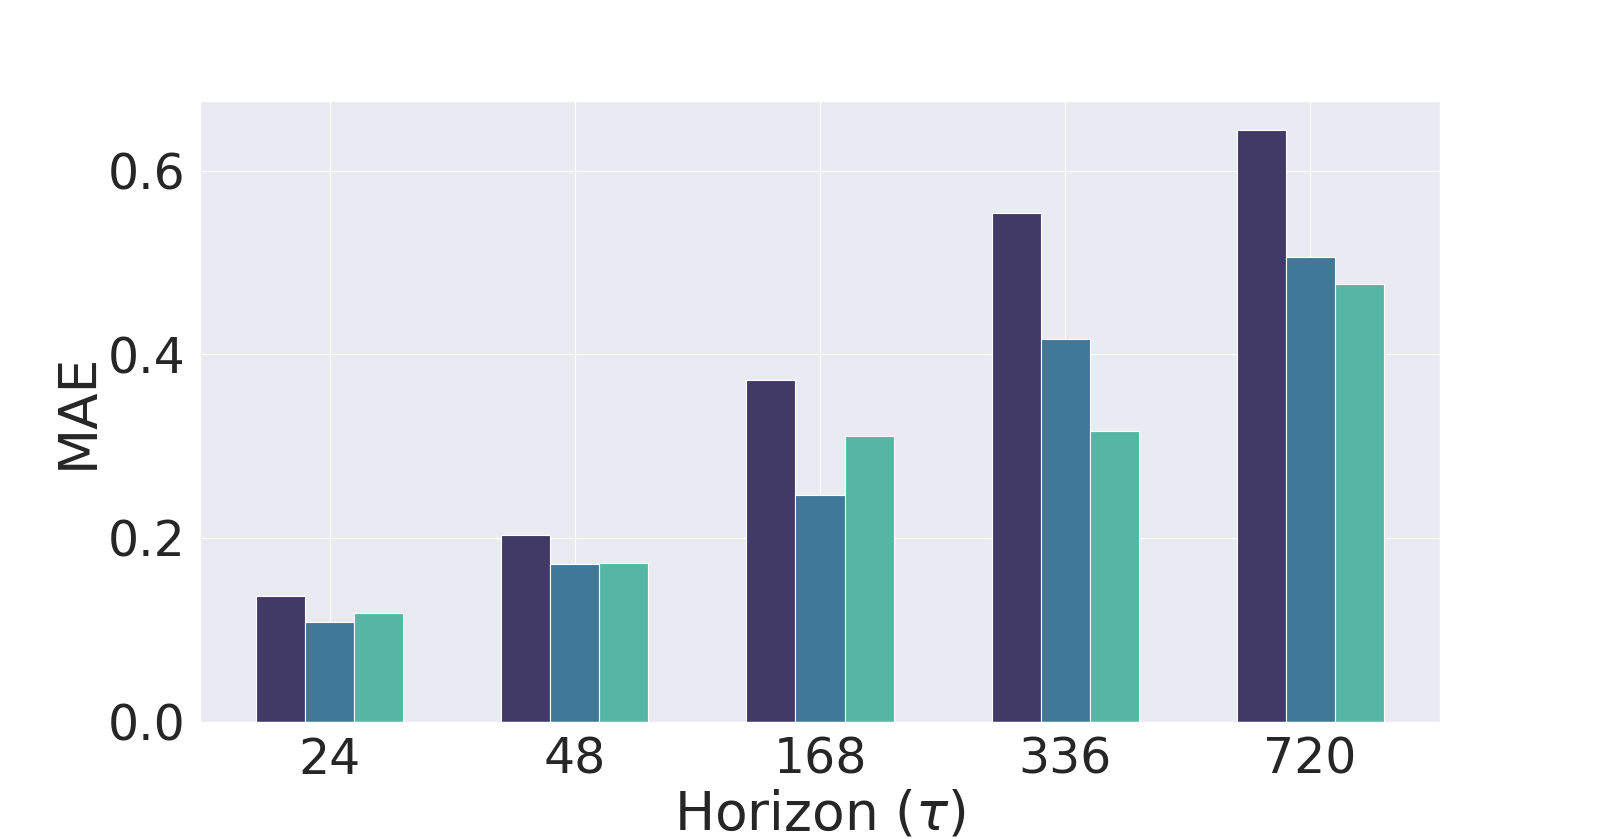
\includegraphics[width=0.40\textwidth]{figs/archi_ablation_uni_ETTm1.png}
    }

    \subfloat[ETTm1 Multivariate\label{fig:ablation_archi_multi}]{%
      \includegraphics[width=0.40\textwidth]{figs/archi_ablation_multi_ETTm1.png}
    }
    
    
    \\
    \subfloat[ETTm1 Univariate\label{fig:skipless_ablation_uni}]{%
      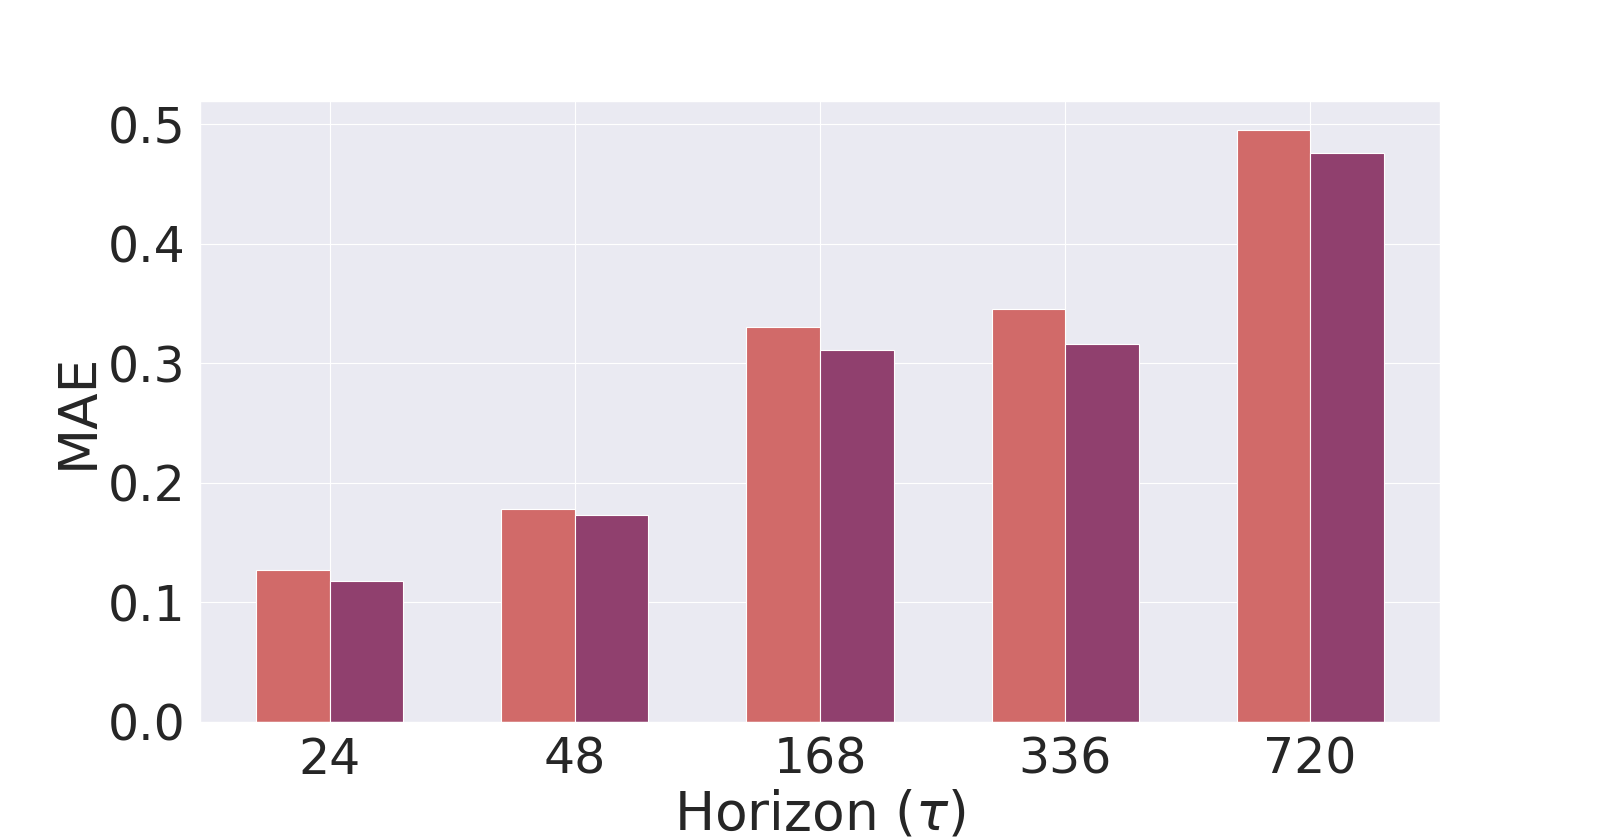
\includegraphics[width=0.40\textwidth]{figs/skipless_ablation_uni_updated.png}
    }
    \subfloat[ETTm1 Multivariate\label{fig:skipless_ablation_multi}]{%
      \includegraphics[width=0.40\textwidth]{figs/skipless_ablation_multi_updated.png}
    }
    \end{tabular}
\caption{(top) Figures \ref{fig:ablation_archi_uni}, \ref{fig:ablation_archi_multi} illustrates the reduction in MAE loss (y-axis) by  the Yformer architecture in comparison with the Informer baseline for the univariate and multivariate settings respectively. The Yformer ($\alpha=0$) represent the Yformer architecture without the reconstruction loss. (bottom) Figures \ref{fig:skipless_ablation_uni}, \ref{fig:skipless_ablation_multi} demonstrate the reduction in MAE loss (y-axis) brought by the addition of U-Net based skip connections (Yformer) to the Yformer architecture without the skip connections (Yformer$^*$). }
\label{fig:ablation_archi}
\end{figure}

\subsection{Effectiveness of the U-Net based skip connections}

To analyze the impact of U-Net based skip-connections, we conduct an ablation study on the Y-former architecture by removing the U-Net skip connections from the encoder to the decoder. We denote this model as Yformer$^*$. Figures \ref{fig:skipless_ablation_uni}, \ref{fig:skipless_ablation_multi} provides a summary of the results obtained after hyperparameter tuning the Yformer$^*$ and comparing it with the proposed Yformer model. The skip connections from the encoder to the decoder improve the performance throughout the entire horizon range for the multivariate setting and offers partial improvement for the univariate setting. Within the multivariate setting, the skip connections have a considerable impact on larger horizons and a smaller impact on the shorter horizons. This observation can be reasoned by considering the fact that long-range forecasting can utilize the additional multi-resolution encoder feature maps encoded by the U-Net based skip connections. Similar reason can be applied to the fact that U-Net based skip connections improve the performance of the multivariate setting more than that of the univariate settings.

\subsection{Reconstruction Factor}
\begin{figure}[t]
    \centering
    \begin{tabular}{c}
    \subfloat[best $\alpha$'s for Univariate\label{fig:alpha_ablation_uni}]{%
      \includegraphics[width=0.33\textwidth]{figs/factor_ablation_uni.png}
    }
    \subfloat[best $\alpha$'s for Multivariate\label{fig:alpha_ablation_multi}]{%
      \includegraphics[width=0.33\textwidth]{figs/factor_ablation_multi.png}
    }
    \subfloat[Model complexity\label{fig:model_size_comparison}]{%
      \includegraphics[width=0.34\textwidth]{figs/model_size_comparison.png}
    }
    \end{tabular}
\caption{Figures \ref{fig:alpha_ablation_uni} and \ref{fig:alpha_ablation_multi} illustrates the distribution of selected Reconstruction factor (y-axis) across the multiple horizons (x-axis). Figure \ref{fig:model_size_comparison}, compares the model size complexity (y-axis) for the multivariate setting across the multiple horizons (x-axis) for the Informer and the Yformer model.}
\label{fig:alpha_ablation}
\end{figure}


How impactful is the reconstruction factor $\alpha$ from the proposed loss in Eq. \ref{eqn:reconstruction}? We aggregated the optimal value chosen by hyperparameter tuning $\alpha$ across different datasets and summarized the distribution in Figures \ref{fig:alpha_ablation_uni} and \ref{fig:alpha_ablation_multi}. 
Interestingly, $\alpha$ value of $0.7$ is the predominant optimal setting across most horizons. Consequently, this shows that a high weight for the reconstruction loss helps the Yformer to achieve a lower loss for the future targets. Moreover, we can observe a trend that $\alpha$ is on average larger for short forecasting horizons signifying the importance of auxiliary loss for the shorter horizons. One possible reason could be that the reconstruction loss generalizes the output distribution better and avoids overfitting on short-horizon lengths. For the longer horizon forecasts, optimal $\alpha$ values are distributed on the lower and upper range of $\alpha$'s evenly, indicating that for long horizons, the reconstruction loss from long history helps for some datasets and does not for other datasets. This could be a characteristic of the dataset having a domain shift within the forecast horizon.


}
\fi

We evaluate the impact of different settings on the performance of FLEX using various ablation tests. 
\Cref{tab:fusion_arch} compares different multi-view fusion architectures.  
% Notice there is a 2mm performance improvement using our multi-head attention layer. 
Note that using attention rather than convolution yields a 2mm improvement.
The performance degrades with the transformer encoder due to its large number of parameters, which require more data for training than what is available in our case.

\Cref{tab:num_views} measures MPJPE on Human3.6M in several studies.
\Cref{tab:num_views}(a) studies a varying number of views, where the 2D pose is once given and once estimated. It confirms that a larger number of views induces more accurate results. Note that the gap between the two columns decreases once the number of views increases. It shows that using several views compensates for the inaccuracy of estimated 2D poses. 
%
\Cref{tab:2D_backbone}(b) compares 2D pose estimation backbones, and justifies our use of Iskakov \etal~\cite{iskakov2019learnable}.
%. It justifies using the pose estimation used by Iskakov \etal~\cite{iskakov2019learnable} as our 2D pose backbone. 
%
Finally, in \Cref{tab:ablation}(c) we explore
% measure our network performance using 
two variations, both with ground-truth 2D inputs. 
The first variation runs FLEX as a monocular method (K=1) and averages the monocular predictions.
%, and show that it yields results that are inferior to fusing the views by our network. 
%
The second changes the fusion layers, $F_S$ and $F_Q$, to use late fusion instead of an early one. 
We conclude that the configuration used by FLEX is better than both variations.
%We find that early fusion works better in our setting. 
% All models use ground-truth 2D poses. 

\begin{wrapfigure}{R}{0.5\textwidth}
\centering

\setlength{\abovecaptionskip}{-32pt plus 3pt minus 2pt}
\setlength{\belowcaptionskip}{0pt plus 3pt minus 2pt}
\caption*{}
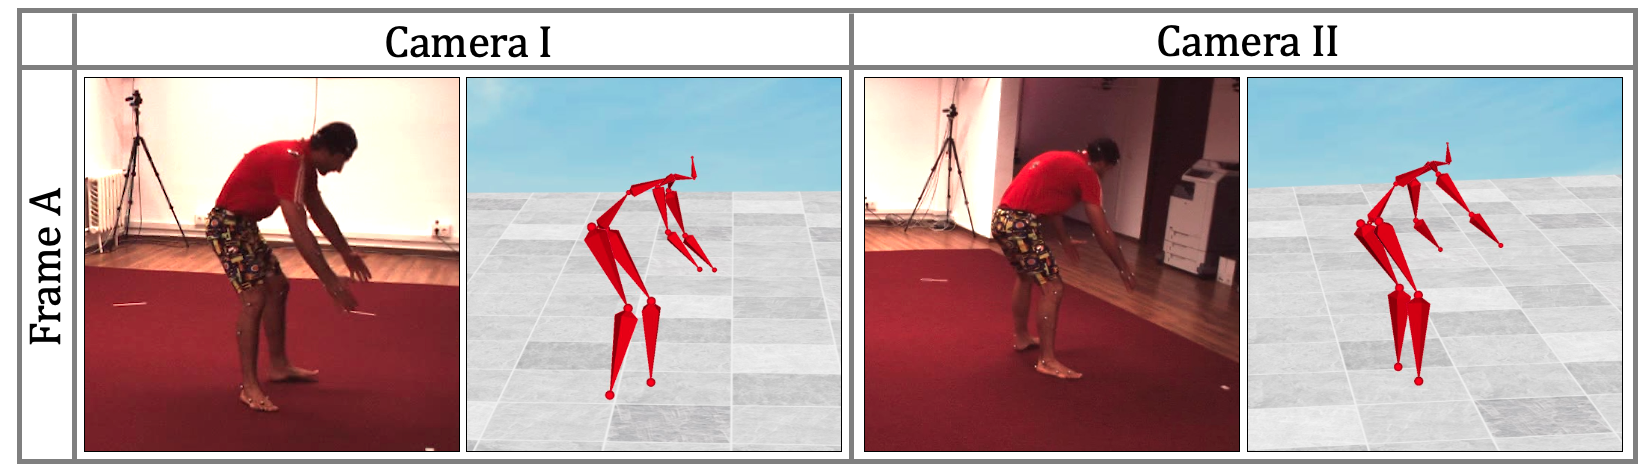
\includegraphics[width=0.5\textwidth]{./images/rebutall_2cams_b.png}

\setlength{\abovecaptionskip}{-33pt plus 3pt minus 2pt}
\setlength{\belowcaptionskip}{0pt plus 3pt minus 2pt}
\caption*{}
\label{fig:generalization_inset}

\end{wrapfigure}

\setcolor{violet}
\paragraphtinyvert{Generalization}
%
% The evaluation on the KTH Football dataset and the synthetic videos
% is done with a model trained on Human3.6M, demonstrating generalization.
%
% We demonstrate  \\ generalization by training on one dataset, Human3.6M, and evaluating on a different, more challenging, dataset, KTH Football, and on the synthetic videos.
We exhibit generalization by training on one dataset and evaluating on a different, more challenging one. The train dataset is Human3.6M, and the evaluation ones are the KTH Football dataset, and the synthetic videos.
%
%In \Cref{fig:football_teaser} and in the sup. mat. we show results in which FLEX was trained on the Human3.6M dataset and evaluated on the Football dataset.
For quantitative measurement, we train our model on two of the four cameras of the Human3.6M dataset.
We test it using the other two cameras, on which the model has not been trained. 
We repeat this process for all possible camera pairs and obtain an average MPJPE of 148mm. Note that this error is not large compared to the human body size, and indeed we attain pleasing visual results as shown in the inset on the right.
\setcolor{black}

